%%%%%%%%%%%%%%%%%%%%%%%%%%%%%%%%%%%%%%%%%%%
%%% DOCUMENT PREAMBLE %%%
%This template was adapted from a template by Roza Aceska.
\documentclass[12pt]{report}
\usepackage[english]{babel}
%\usepackage{natbib}
\usepackage{url}
\usepackage[utf8x]{inputenc}
\usepackage{amsmath}
\usepackage{graphicx}
\usepackage{parskip}
\usepackage{fancyhdr}
\usepackage{vmargin}
\usepackage{caption}
\usepackage{subcaption}
\setmarginsrb{3 cm}{2.5 cm}{3 cm}{2.5 cm}{1 cm}{1.5 cm}{1 cm}{1.5 cm}

\title{Report Assignment Part 1}								
% Title
\author{}						
% Author
\date{}
% Date

\makeatletter
\let\thetitle\@title
\let\theauthor\@author
\let\thedate\@date
\makeatother

\pagestyle{fancy}
\fancyhf{}
\rhead{\theauthor}
\lhead{\thetitle}
\cfoot{\thepage}
%%%%%%%%%%%%%%%%%%%%%%%%%%%%%%%%%%%%%%%%%%%%
\begin{document}

%%%%%%%%%%%%%%%%%%%%%%%%%%%%%%%%%%%%%%%%%%%%%%%%%%%%%%%%%%%%%%%%%%%%%%%%%%%%%%%%%%%%%%%%%

\begin{titlepage}
	\centering
    \vspace*{0.5 cm}
  \begin{center}    \textsc{\Large   Adavanced Process Mining SS20}\\[2.0 cm]	\end{center}
	\rule{\linewidth}{0.2 mm} \\[0.4 cm]
	{ \huge \bfseries \thetitle}\\
	\rule{\linewidth}{0.2 mm} \\[1.5 cm]
	
  \begin{minipage}{0.48\textwidth}
    \begin{flushleft} \large
      \emph{Submitted To:}\\
      Tobias Brockhoff\\
      Lisa Mannel\\
      Sebastiaan J. van Zelst MSc PhD\\
    \end{flushleft}
  \end{minipage}~
  \begin{minipage}{0.48\textwidth}
    \begin{flushright} \large
			\emph{Submitted By:} \\
      Student 1 (Matr. Number) \\
      Student 2 (Matr. Number) 
		\end{flushright}
	\end{minipage}\\[2 cm]
	
\end{titlepage}

%%%%%%%%%%%%%%%%%%%%%%%%%%%%%%%%%%%%%%%%%%%%%%%%%%%%%%%%%%%%%%%%%%%%%%%%%%%%%%%%%%%%%%%%%

\renewcommand{\thesection}{\arabic{section}}
General notes:
\begin{itemize}
  \item Remove this general note page and the text in \textlangle \textrangle
  \item This report should be at most 20 A4 pages, including the title page 
  \item	Data supporting your claims should be presented in a suitable and comprehensible aggregated form (diagrams, pictures, charts) and not as raw data tables (they can be added in the appendix)
  \item Submit this report as a PDF file
\end{itemize}
\newpage

\section{Q1. Inductive Miner}

As a first step into discovering the model for the event log, a short exploration was carried before the application of the algorithm. This to familiarize ourselves with the provided data. Besides a visualization of the dataset, a report was automatically generated with a data-centered description. Also, a brief analysis on the cardinality of the relation between traces and the \emph{Patient} column, which was found to be 1:1. Lastly, some random traces were visualized.

\paragraph{a)} 

Overall, we can estimate that the patients situation is assessed through an initial exam and, if necessary, 4 different treatments can be applied. In the process tree generated, visible in Figure \ref{fig:figures-q1_a_tree-pdf}, it is possible to identify the exclusive decision made between the discharge of the initial exam and the isolation inform, but the model fails to identify the relation between this decision and the application of the treatments, that certainly must occur only in infected patients.

\begin{figure}[h]
    \centering
    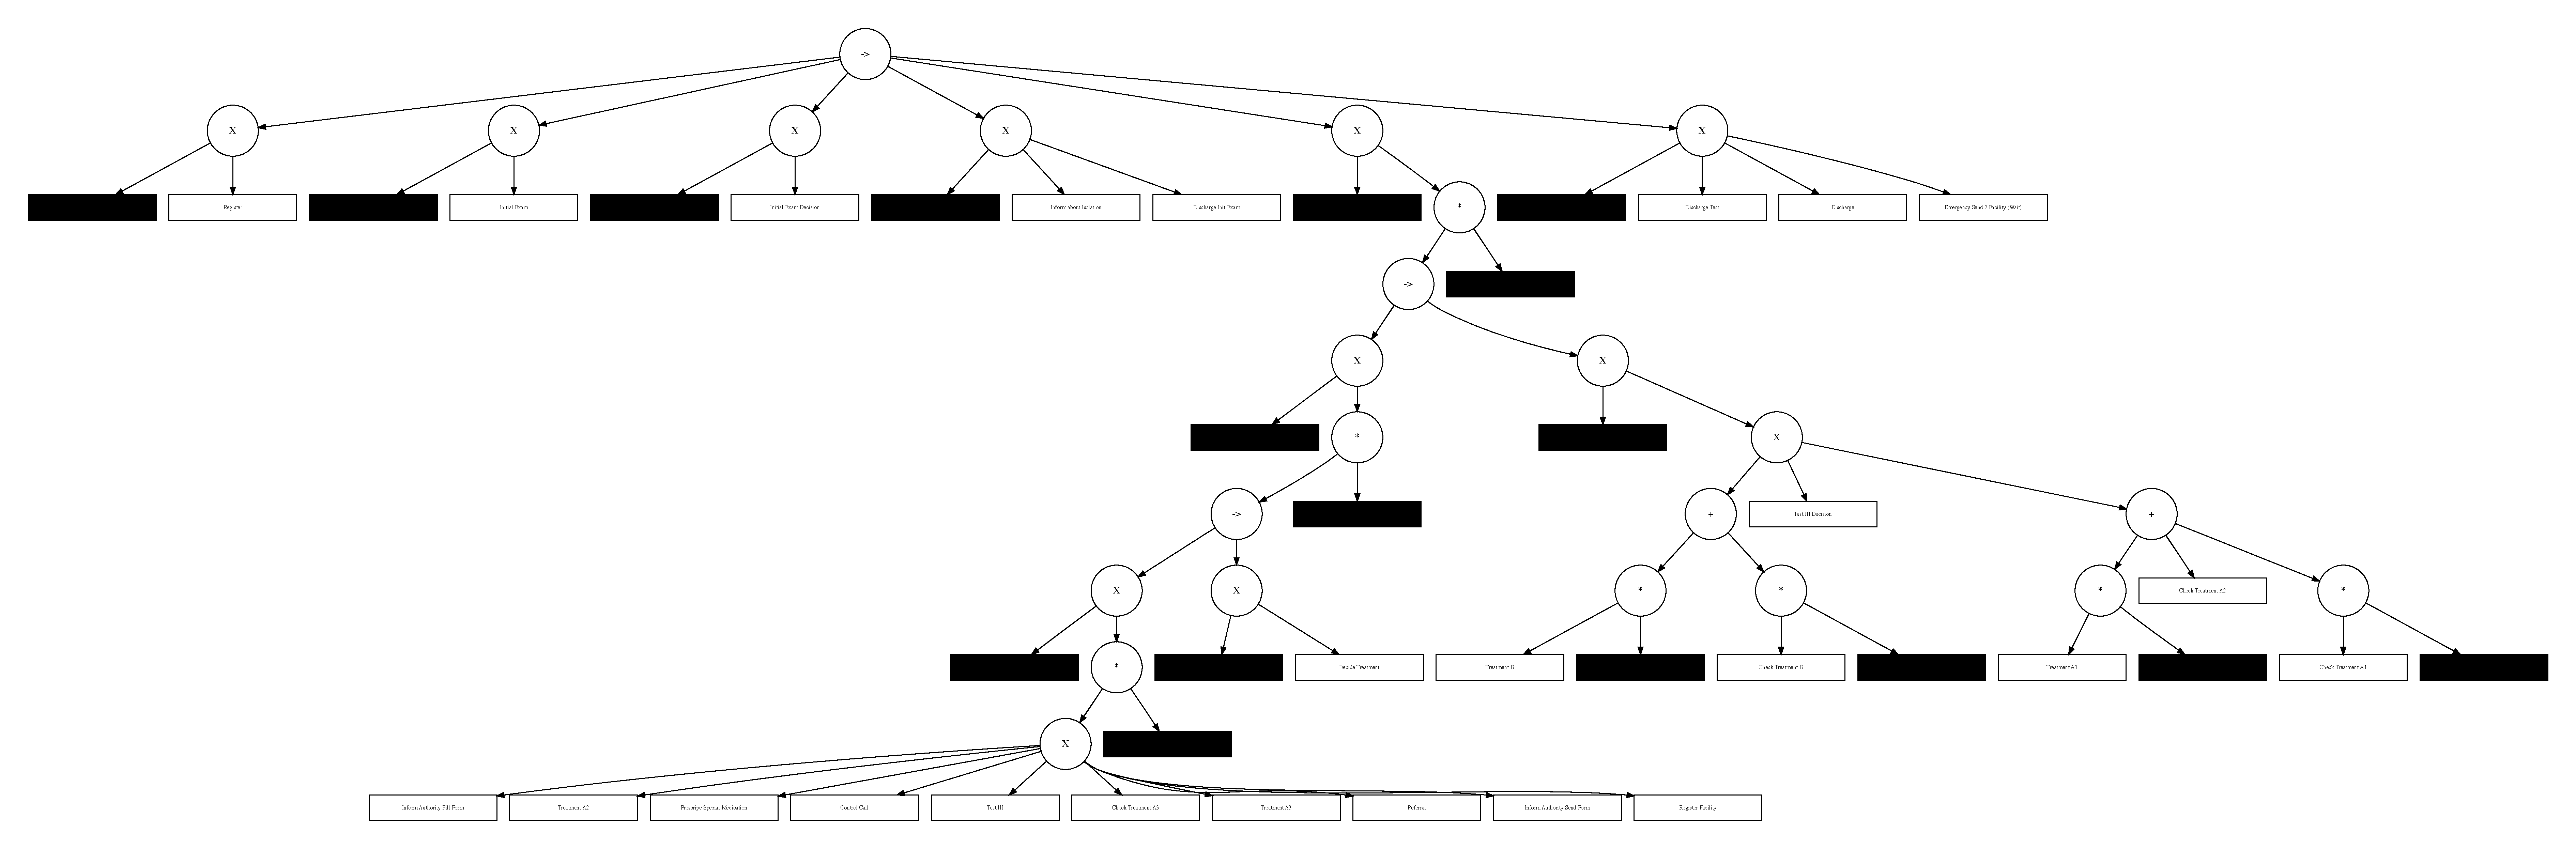
\includegraphics[width=\textwidth]{figures/q1_a_tree.pdf}
    \caption{Process Tree generated by the Inductive Miner}
    \label{fig:figures-q1_a_tree-pdf}
\end{figure}

The treatments are applied multiple times alternating with the respective \emph{Check} activity. Unfortunately, the models are not too helpful in describing the choice of the treatments nor the dynamics of the execution of the remaining activities after the isolation inform. The exceptions are the ending activities, which tells us that the patients can either be discharged or sent to emergency care.

We notice the Inductive Miner guarantee for perfect fitness in the generated model through the presence of several silent transitions, an known outcome of the algorithm mainly present in the outcome of noisy event logs. Another characteristic of the IM is its inability to capture non-local dependencies, as it is shown more obviously, as already mentioned, by the lack of relation between the result of the initial exam and the applications' of the treatments. A more subtle consequence of this characteristic is the inability to constrain the `Check Treatment *` activities to follow, not necessarily directly, the respective treatment activity.

Regarding its precision, we notice there are several characteristics of the process that the model is unable to represent, using underfitting approaches instead. Besides the two mentioned just above, we point out the flower structure in the lowest level of the process tree and the more abstract flower pattern in the second-last exclusive choice operator of the second level. Therefore, we can say that the generated model is perfectly fit to the log, as expected, but not very precise.

The two main reasons identified for the lack of preciseness are the excess of silent transitions and the use of generalist structures (flower pattern). We can estimate that the first may be caused by noise in the data, which is usual. The second can be caused by a limitation of the algorithm, that is unable to deal with non-local dependencies.

\paragraph{b)} 

After distinguishing the two instances of the \emph{Control Call} activity in the event log, the Inductive Miner was again applied and the resulting model can be seen in Figure \ref{fig:figures-q1_b_tree-pdf} below.

\begin{figure}[h]
    \centering
    
\includegraphics[width=\textwidth]{figures/q1_b_tree.pdf}
    \caption{Process Tree after \emph{Control Call} splitting}
    \label{fig:figures-q1_b_tree-pdf}
\end{figure}

We can see that not only the `Control Call` activity was removed from the flower structure at the bottom, but also the `Test III` and `Test III Decision` were brought up to the first sequence operator, of course still within a exclusive-choice operator with a silent activity, due to the noise on the data.

Still, now it is possible to extend our assumptions about the process. After the initial exam proceedings, several control calls can be performed and they are followed by the \emph{Test III}, which defines if the patient will need treatment.

\paragraph{c)} 

After filtering the DFG we can already notice an improvement. The absence of many of the edges in the original DFG made the filtered one much more linear and readable. Still, we can also notice the structure of the activities related to the A treatments is not properly captured. The two DFGs can be seen in Figure \ref{fig:dfg-filtering}.

\begin{figure}[h]
    \centering
    \begin{subfigure}[b]{0.4\textwidth}
	\centering
	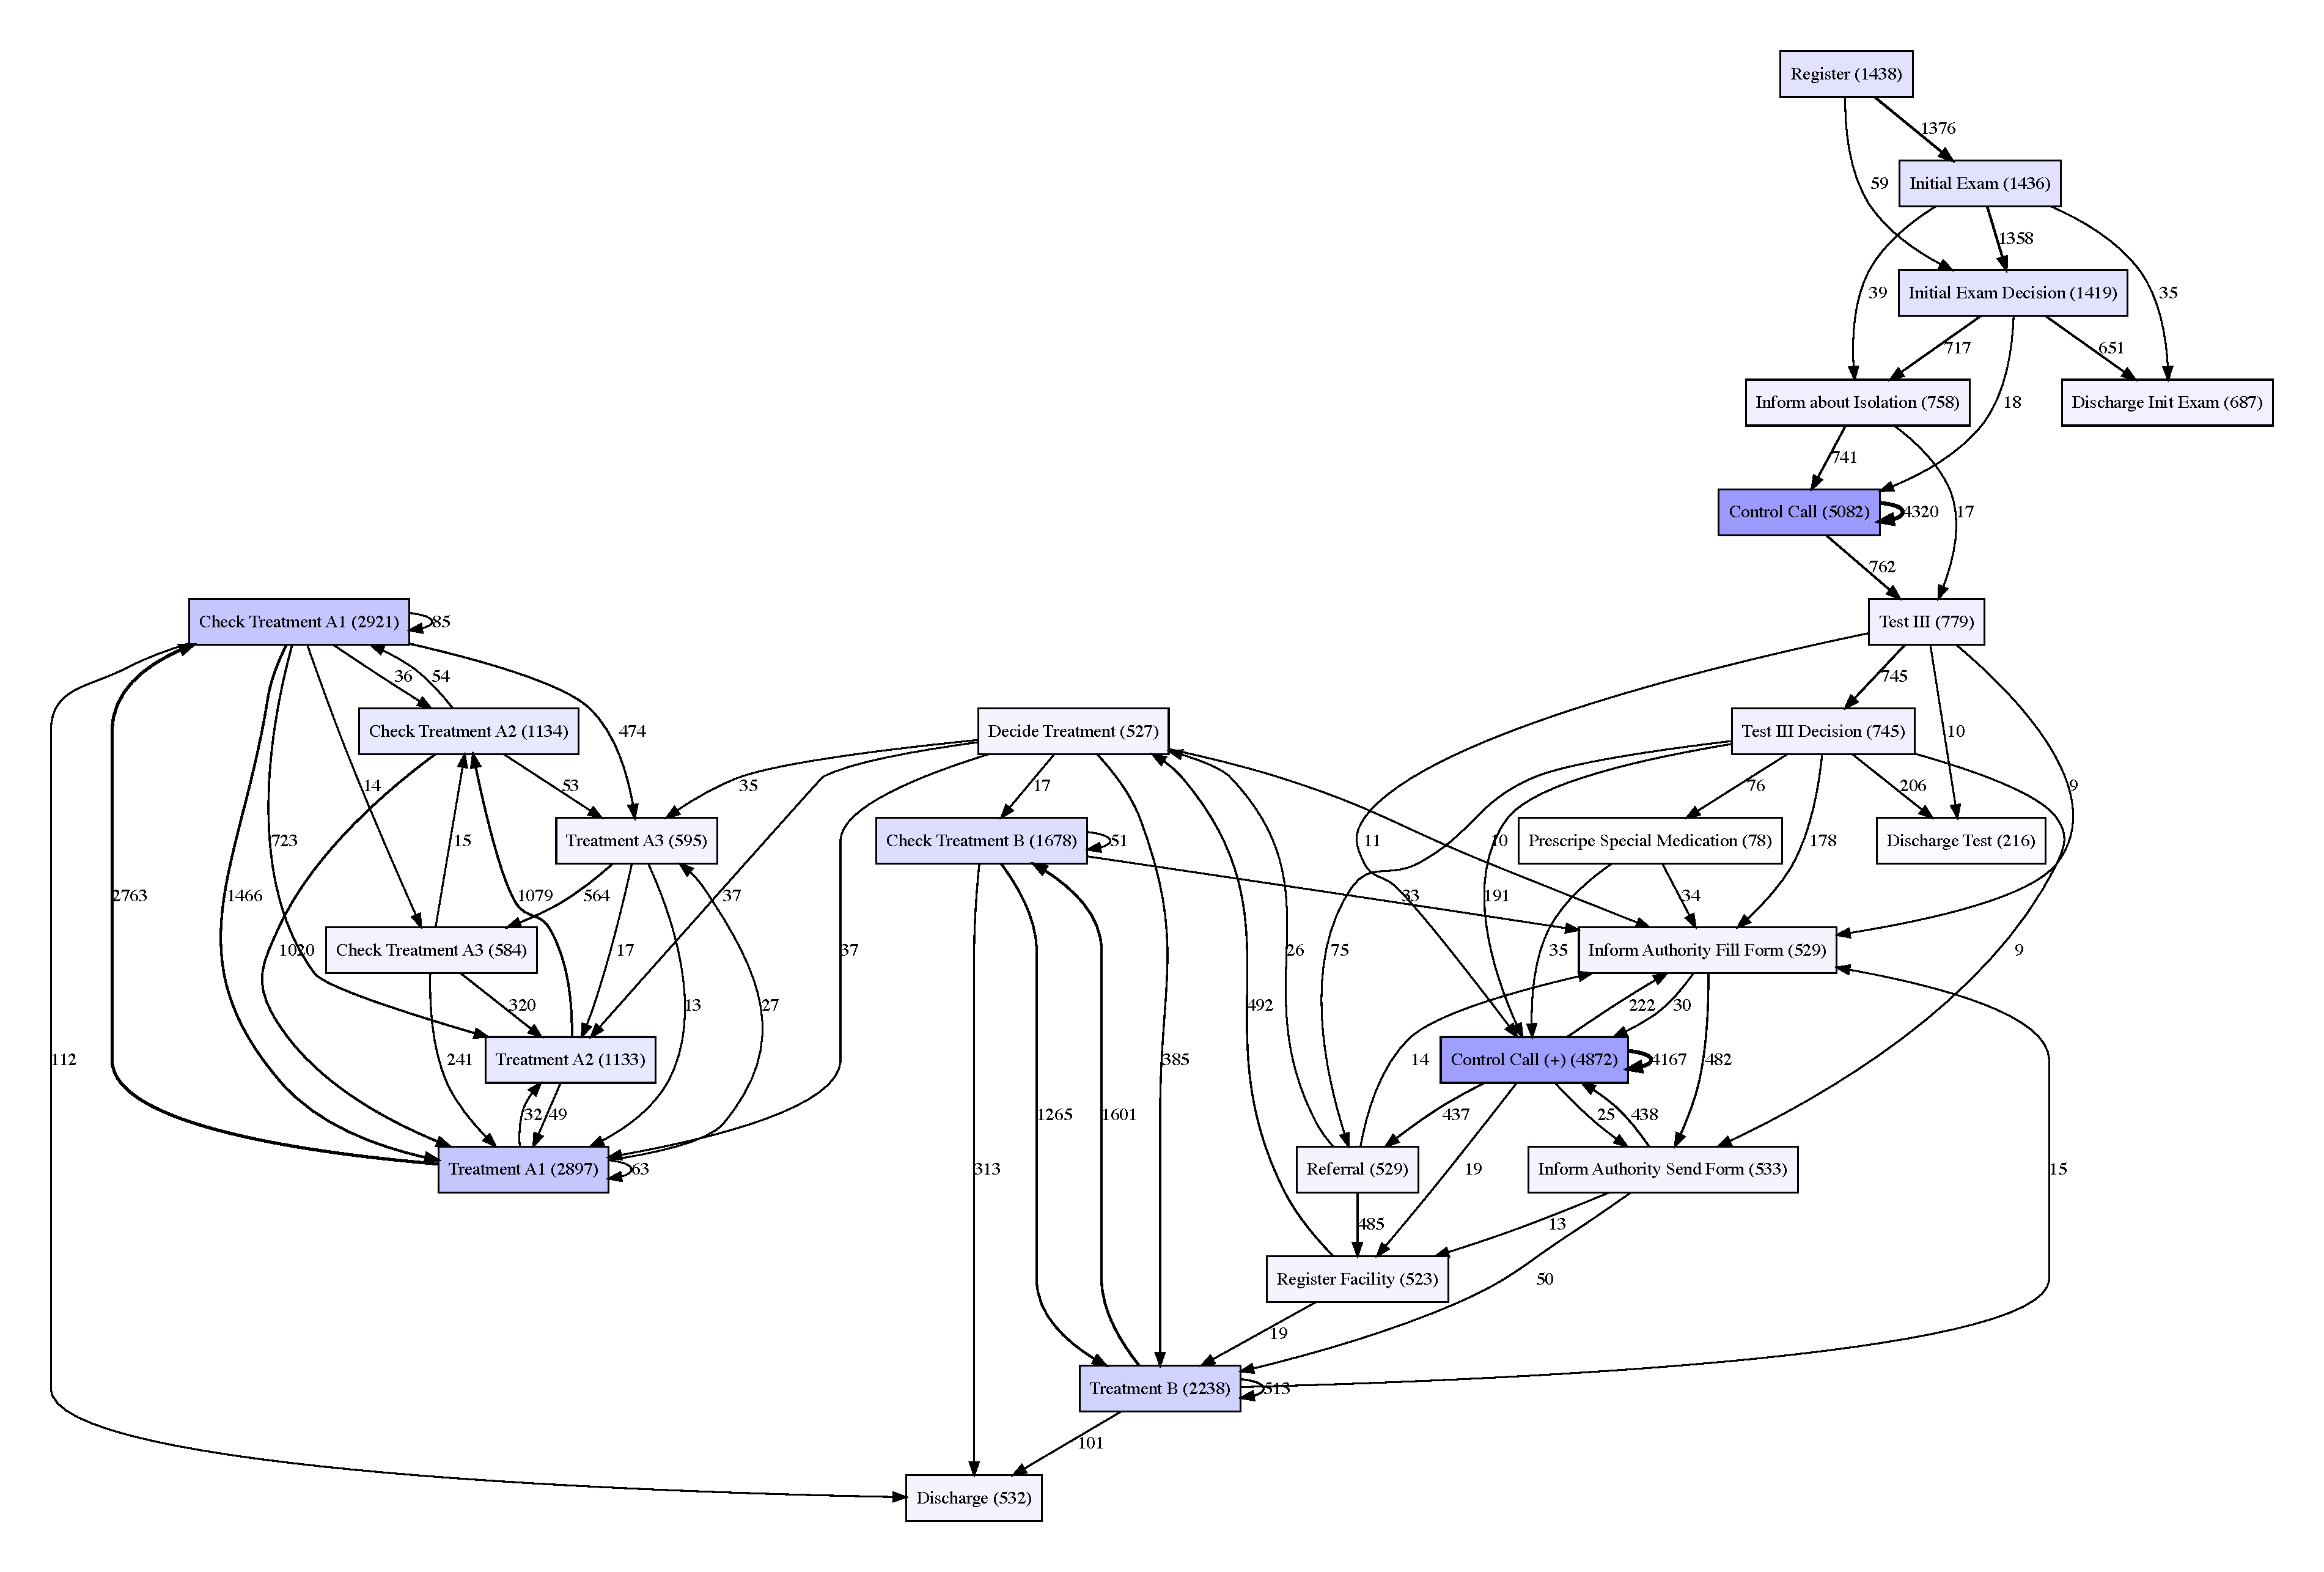
\includegraphics[width=\textwidth]{figures/q1_c_dfg_renaming.pdf}
	\caption{DFG generated after context-sensitive renaming}
	\label{fig:subfigures-q1_c_dfg_renaming-pdf}
    \end{subfigure}
    \hfill
    \begin{subfigure}[b]{0.4\textwidth}
	\centering
	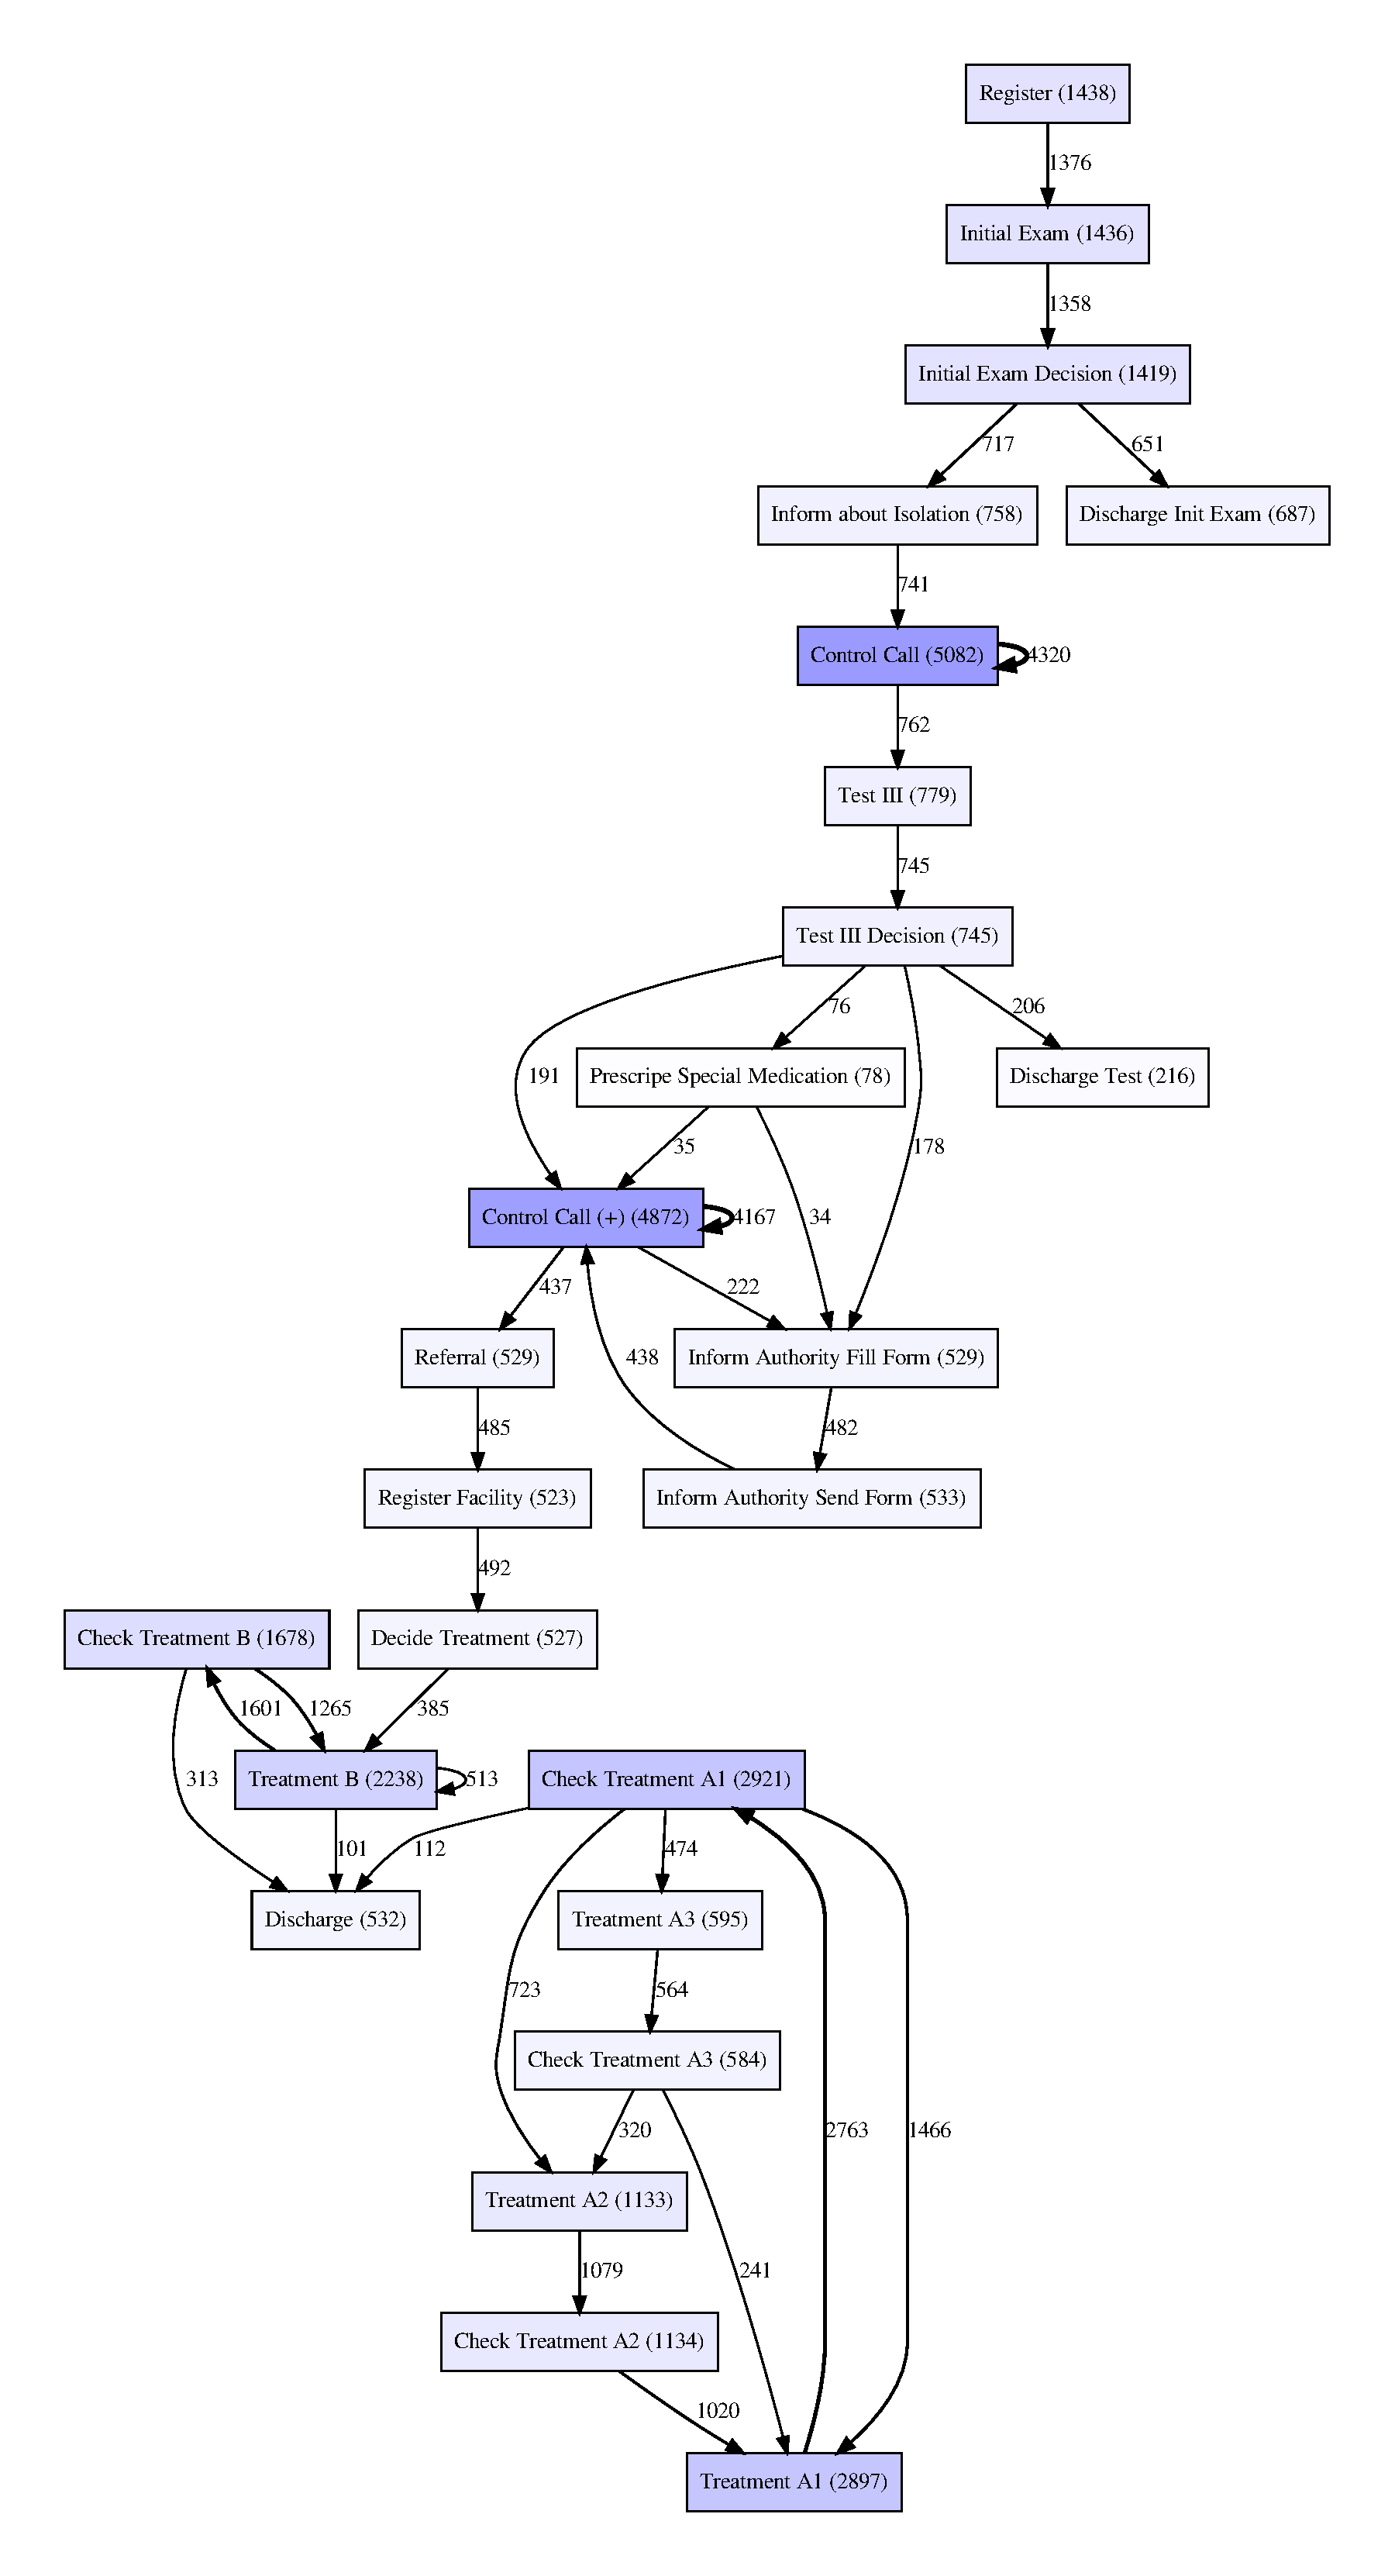
\includegraphics[width=\textwidth]{figures/q1_c_dfg_filtered.pdf}
	\caption{Filtered DFG}
	\label{fig:subfigures-q1_c_dfg_filtered-pdf}
    \end{subfigure}
    \hfill
    \caption{DFG filtering}
    \label{fig:dfg-filtering}
\end{figure}

Upon the filtered DFG, the IM algorithm was run once again and the resulting process tree can be seen in Figure \ref{fig:figures-q1_c_filt_tree-pdf}. The new model generated is much closer to the expected from the superficial analysis of the traces. The noise removed comes mostly from skipped activities, that were not logged, as we can notice through the edges in the DFG that were removed.

Still, the structure of the activities related to the treatment A variants was not captured. One can notice in the bottom of the filtered DFG that the nodes related to these treatments are only connected to the remaining of the graph through the \emph{Discharge} activity, which is supposed to be one of the final activities. This implied in the loop operator right next to the \emph{Register} activity in the process tree and the subsequent silent activities. We estimate this problem was caused by the relative rarity (123 out of 1500) of traces in which these activities are performed, but since they are performed several times for each trace, the edges between these activities were not filtered.

\begin{figure}[h]
    \centering
    
\includegraphics[width=\textwidth]{figures/q1_c_filt_tree.pdf}
    \caption{Process tree generated by the IM application on the filtered DFG}
    \label{fig:figures-q1_c_filt_tree-pdf}
\end{figure}

\paragraph{d)} 

Based on the discussed in the previous, we identify two approaches for the problem with the activities related to the A treatments: the first would be to remove them from the log; the second would be to fine tune the filtering threshold so no to remove the edges from the DFG that relate these activities from the others.

Removing these activities we get the model seen in Figure \ref{fig:dfg-pt-no-A}. Even though we had a great improvement in the structures represented caused by the removal of the pending structure as discussed above. Still, the algorithm fails to understand the sequence structure that should have happened after the non-execution of the \emph{Discharge Init Exam} activity, therefore inserts several silent activities along the tree. Other than that, the operators around the \emph{Control Call} activity after the test are not precise as are not as well the operators that deal with the treatment B related activities. 

\begin{figure}[h]
    \centering
    \begin{subfigure}[b]{0.2\textwidth}
        \centering
	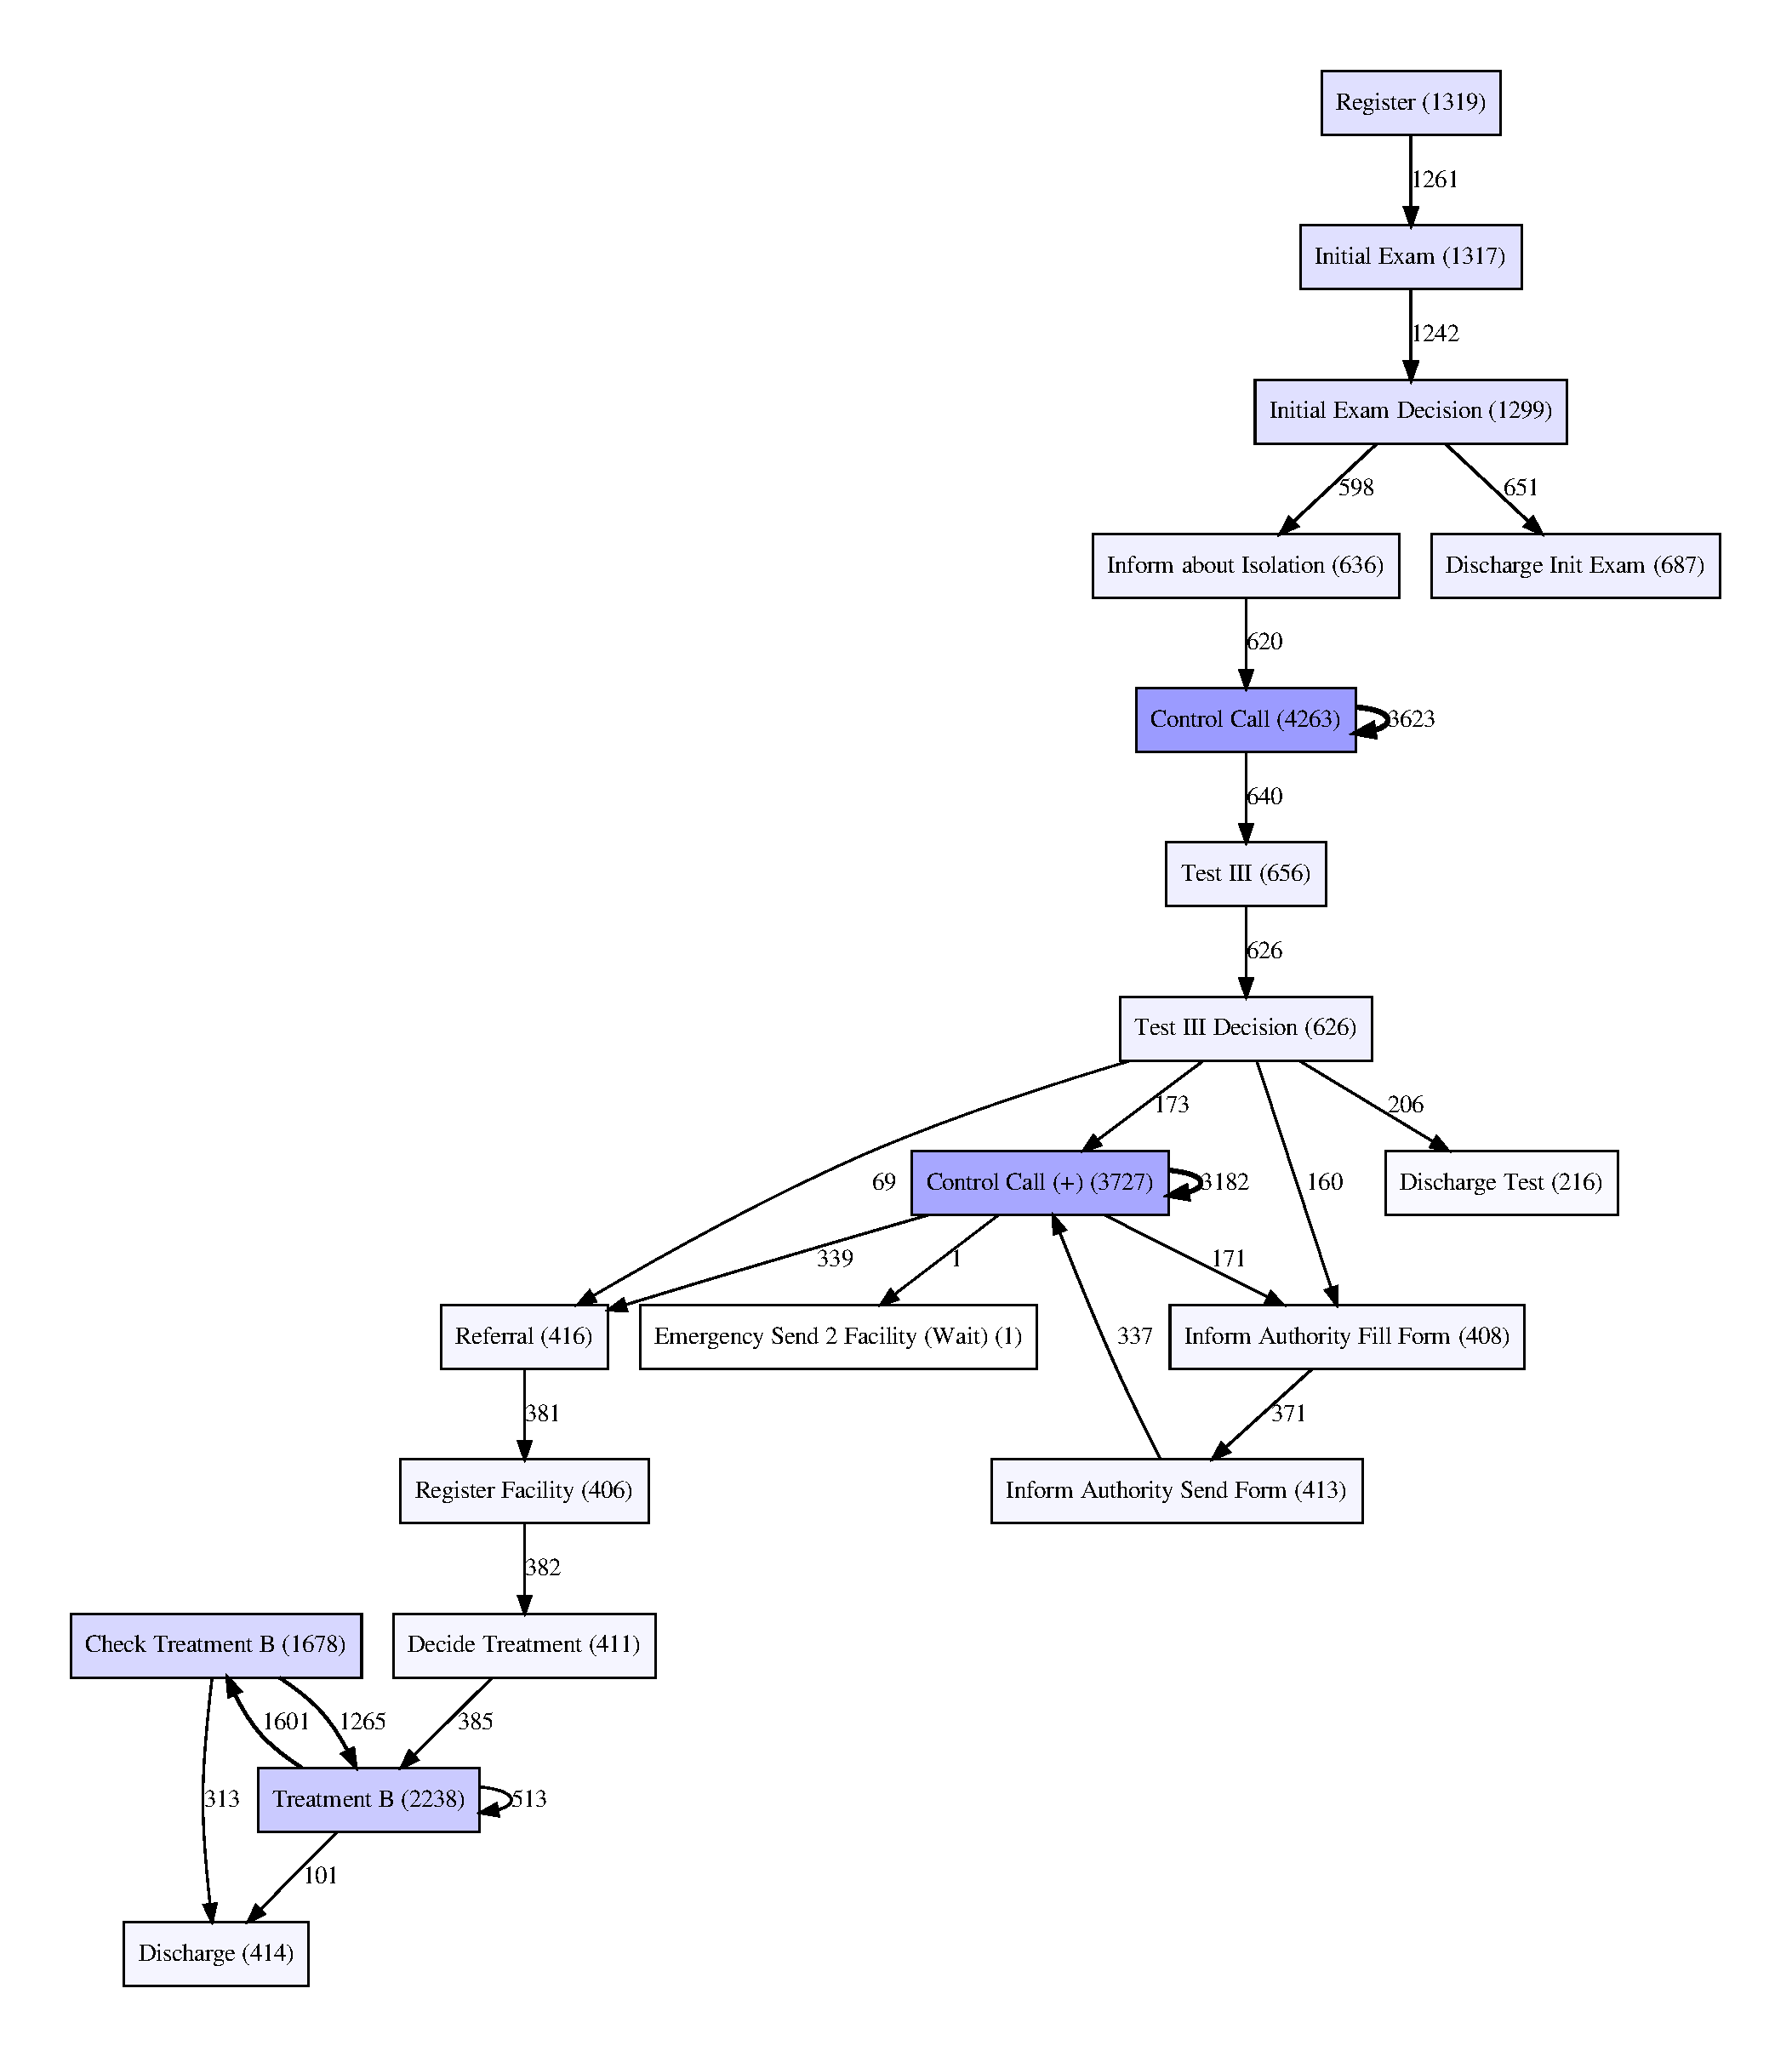
\includegraphics[width=\textwidth]{figures/q1_d_no_A.pdf}
        \caption{DFG}
        \label{fig:figures-q1_d_no_A-pdf}
    \end{subfigure}
    \hfill
    \begin{subfigure}[b]{0.7\textwidth}
        \centering
	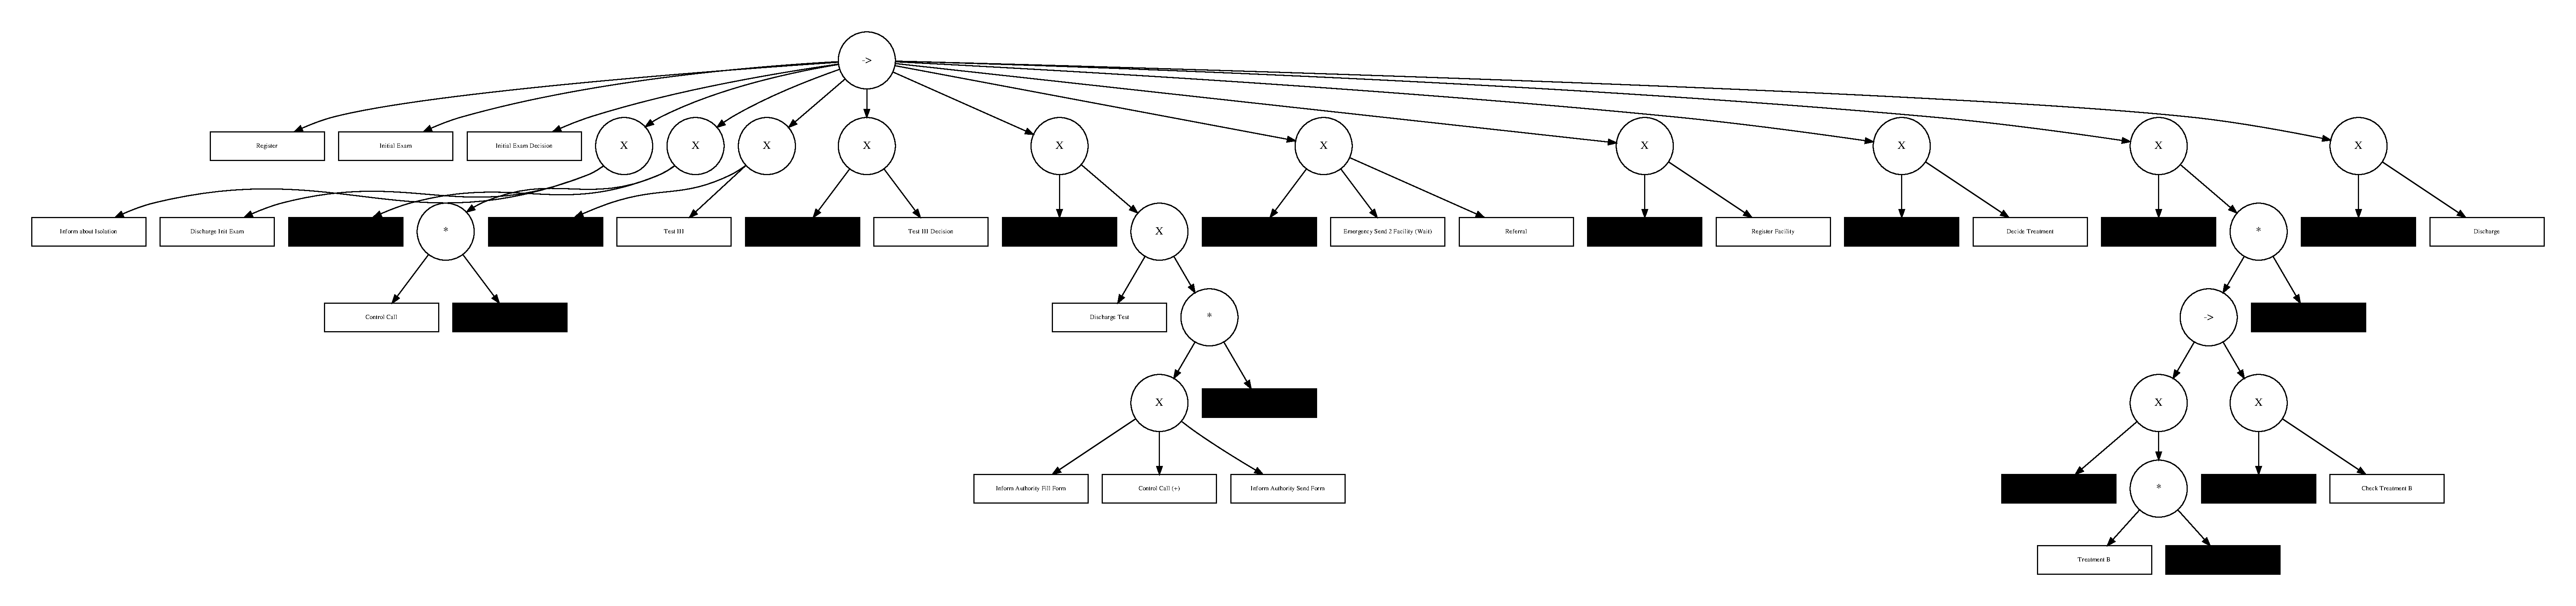
\includegraphics[width=\textwidth]{figures/q1_d_tree_no_A.pdf}
        \caption{Process Tree}
        \label{fig:figures-q1_d_tree_no_A-pdf}
    \end{subfigure}
    \hfill
    \caption{Model resulting after the filtering of the traces containing activities related to the A treatments}
    \label{fig:dfg-pt-no-A}
\end{figure}

A side effect of removing theses traces is that the \emph{Prescripe Special Medication} activity vanished, so we removed just the activities, keeping the traces, which had the precise effect of bringing the mentioned activity back to the model, as can be seen in Figure \ref{fig:dfg-pt-silent-A}.

\begin{figure}[h]
    \centering
    \begin{subfigure}[b]{0.2\textwidth}
        \centering
	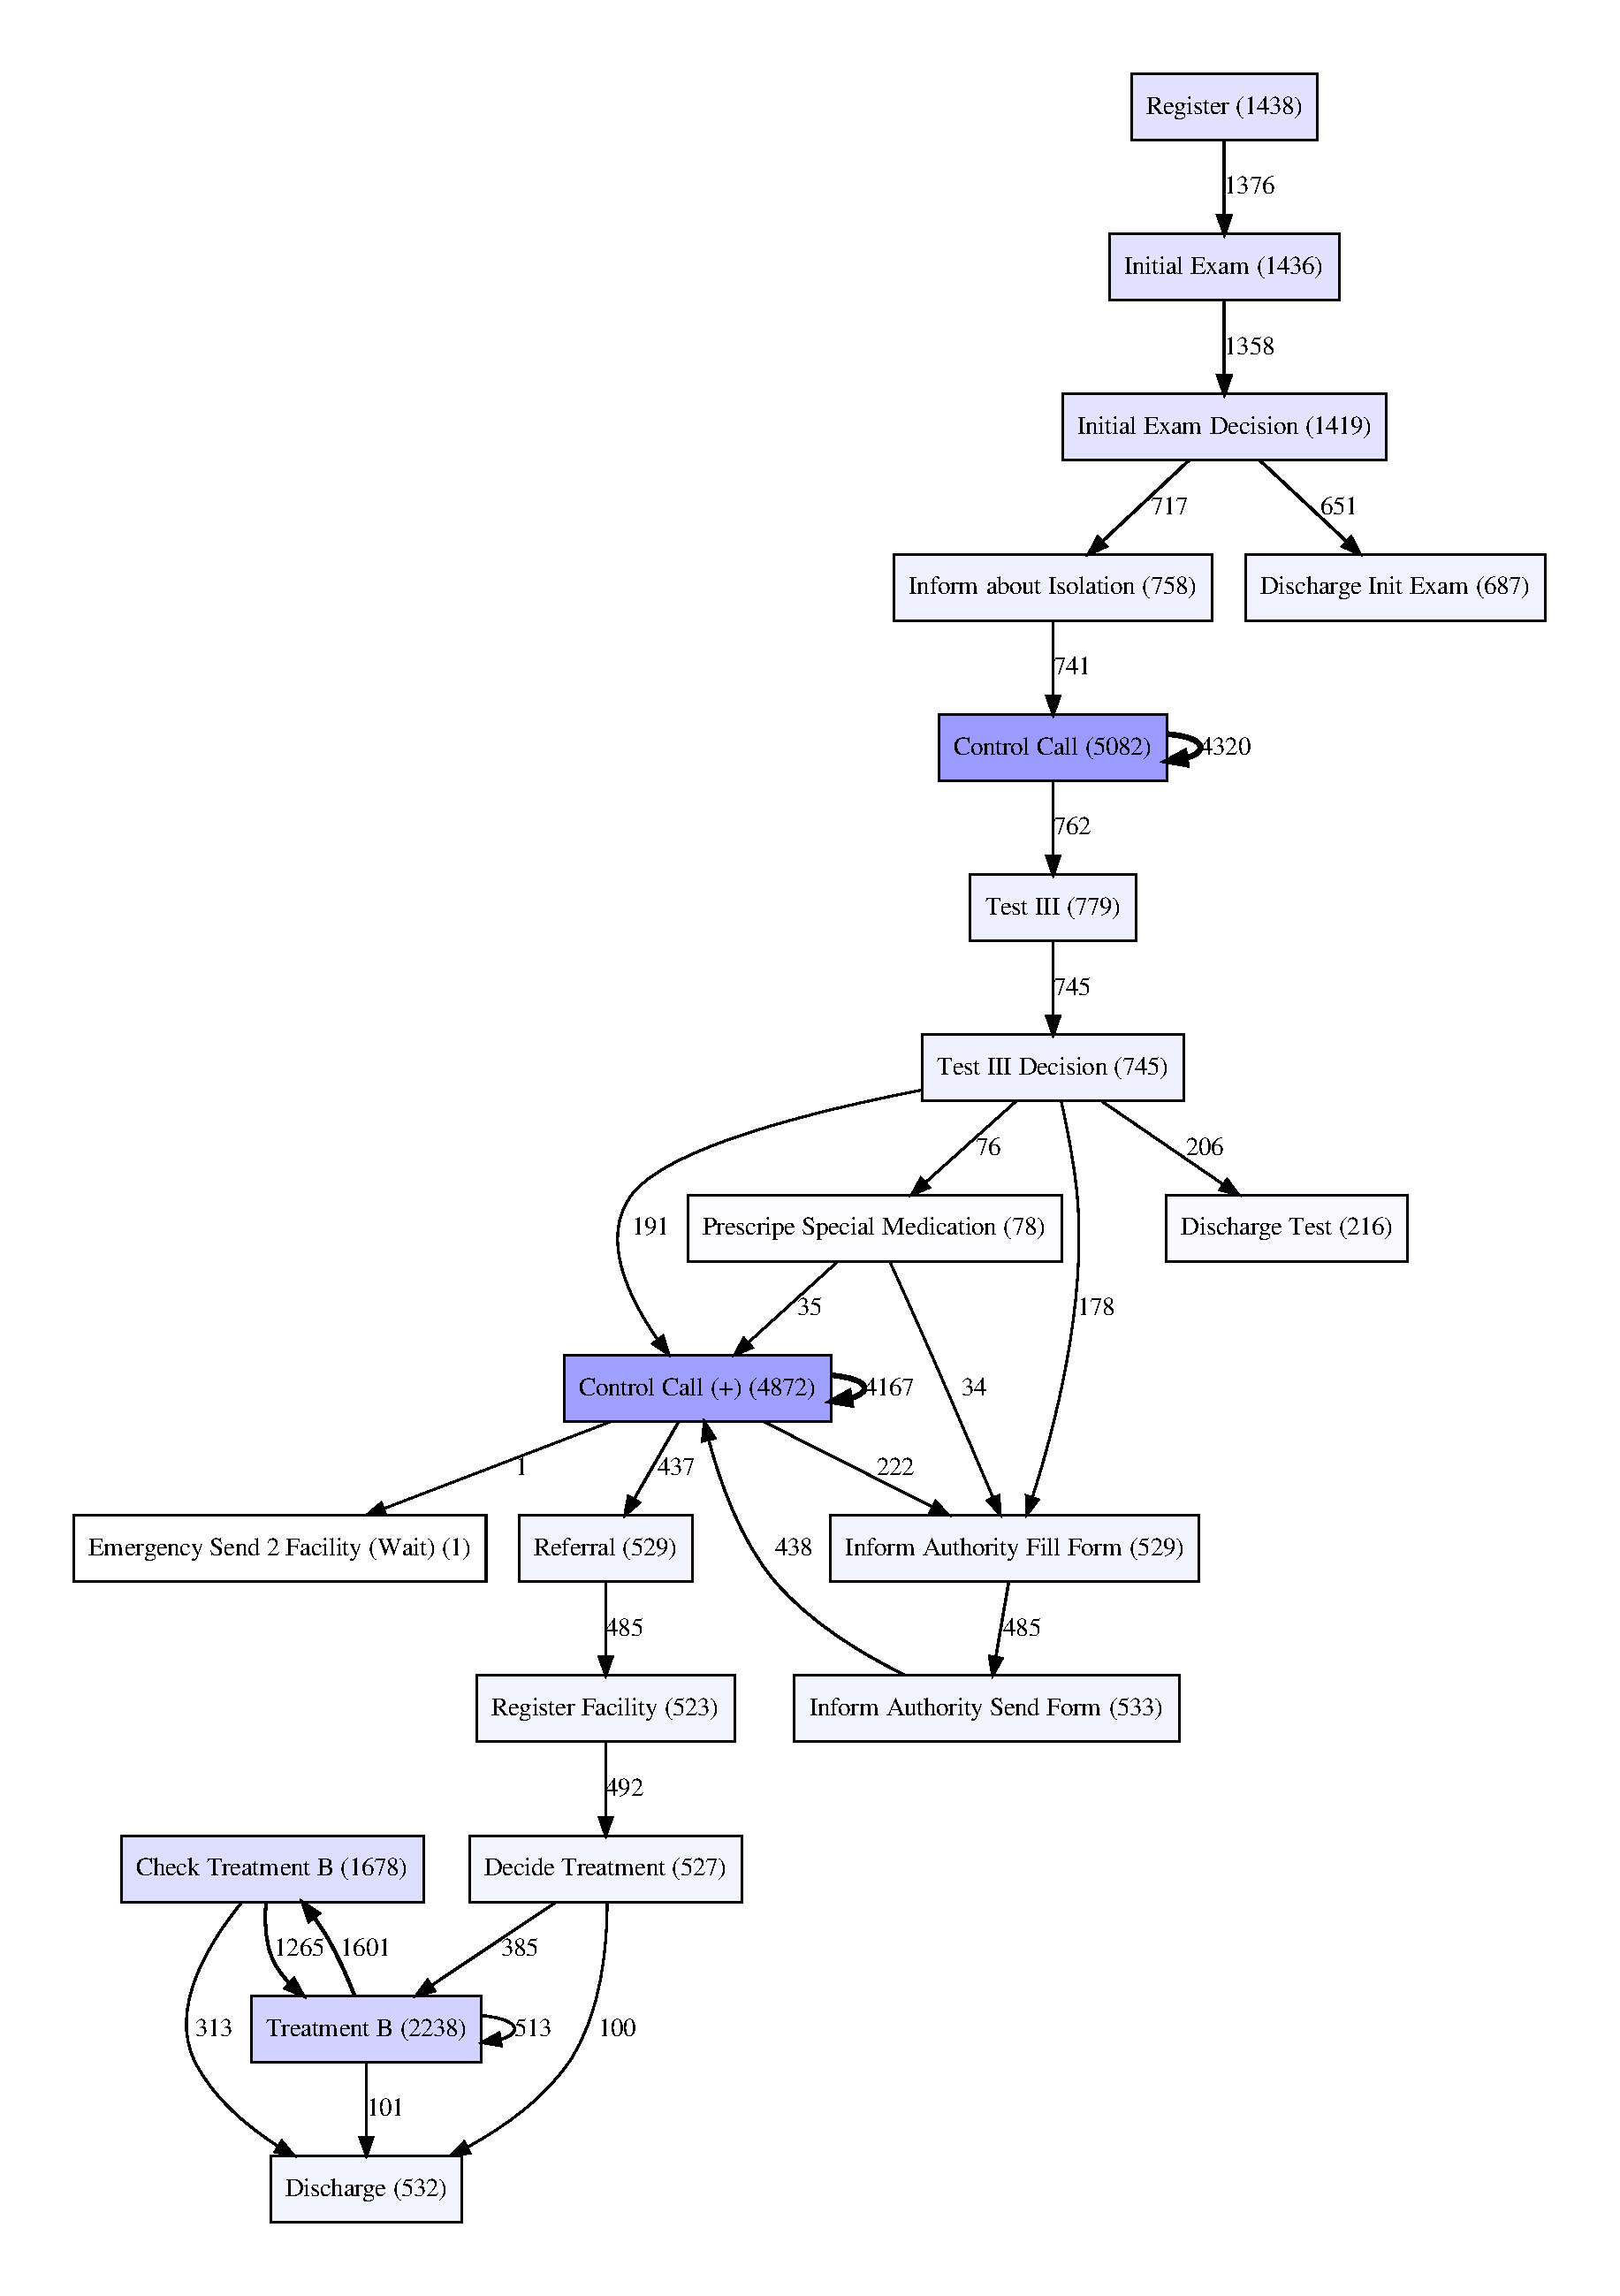
\includegraphics[width=\textwidth]{figures/q1_d_silent_A.pdf}
        \caption{DFG}
        \label{fig:figures-q1_d_silent_A-pdf}
    \end{subfigure}
    \hfill
    \begin{subfigure}[b]{0.7\textwidth}
        \centering
	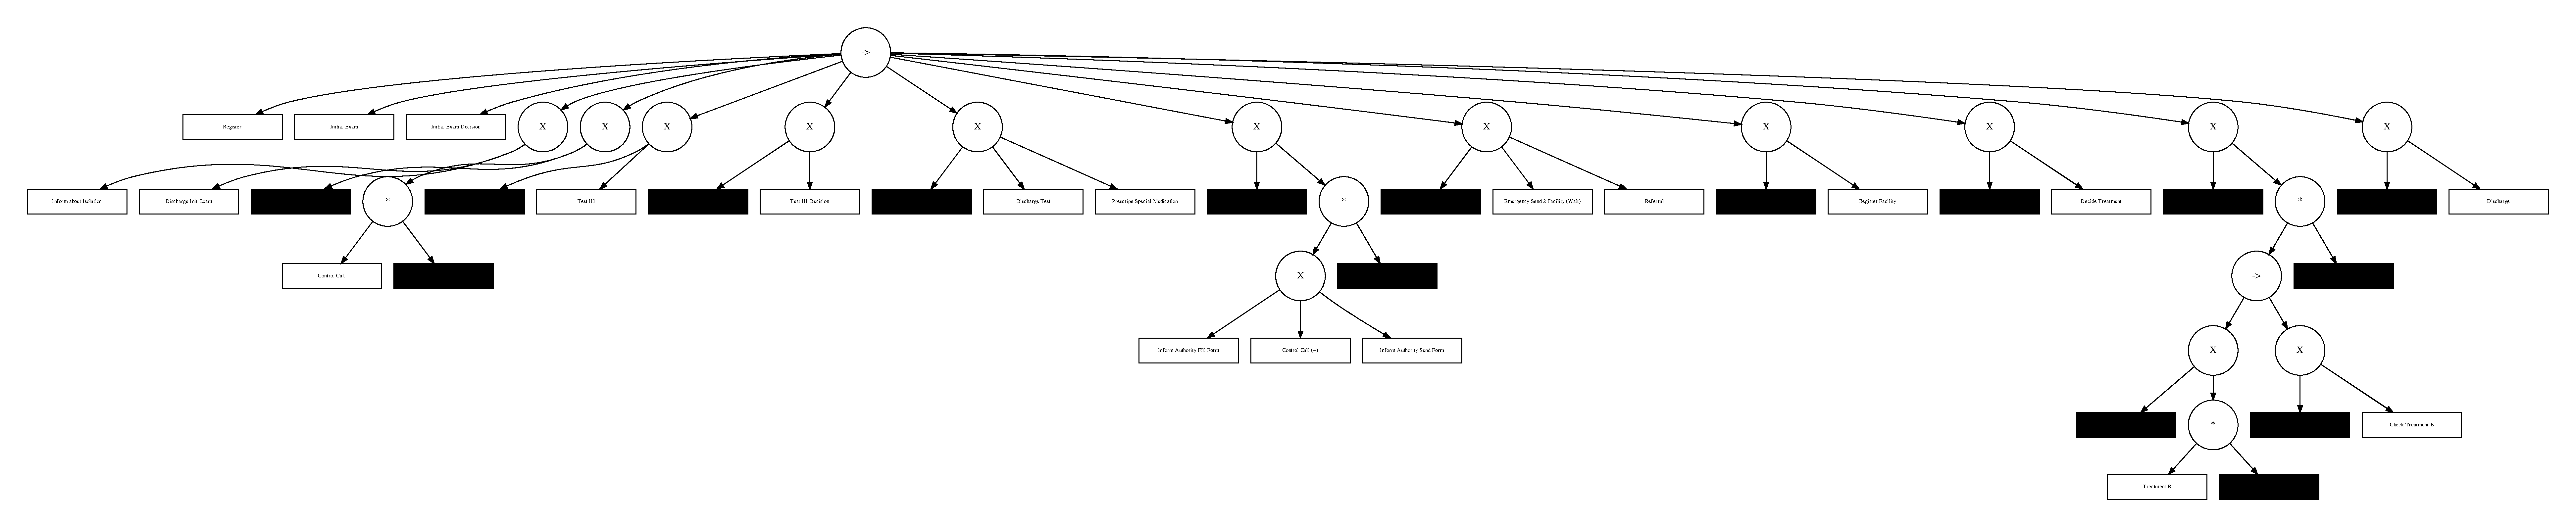
\includegraphics[width=\textwidth]{figures/q1_d_tree_silent_A.pdf}
        \caption{Process Tree}
        \label{fig:figures-q1_d_tree_silent_A-pdf}
    \end{subfigure}
    \hfill
    \caption{Model resulting after the filtering of just the activities related to the A treatments}
    \label{fig:dfg-pt-silent-A}
\end{figure}

The fine tuning of the threshold resulted in the model that can be seen in Figure \ref{fig:noise-threshold-tuning-model}. This approach resulted in a model that represents more behaviors of the event log. The major outcome in the model would be the exclusive choice operator after the \emph{Decide Treatment} activity that distinguished between the treatments.

\begin{figure}[h]
    \centering
    \begin{subfigure}[b]{0.2\textwidth}
        \centering
	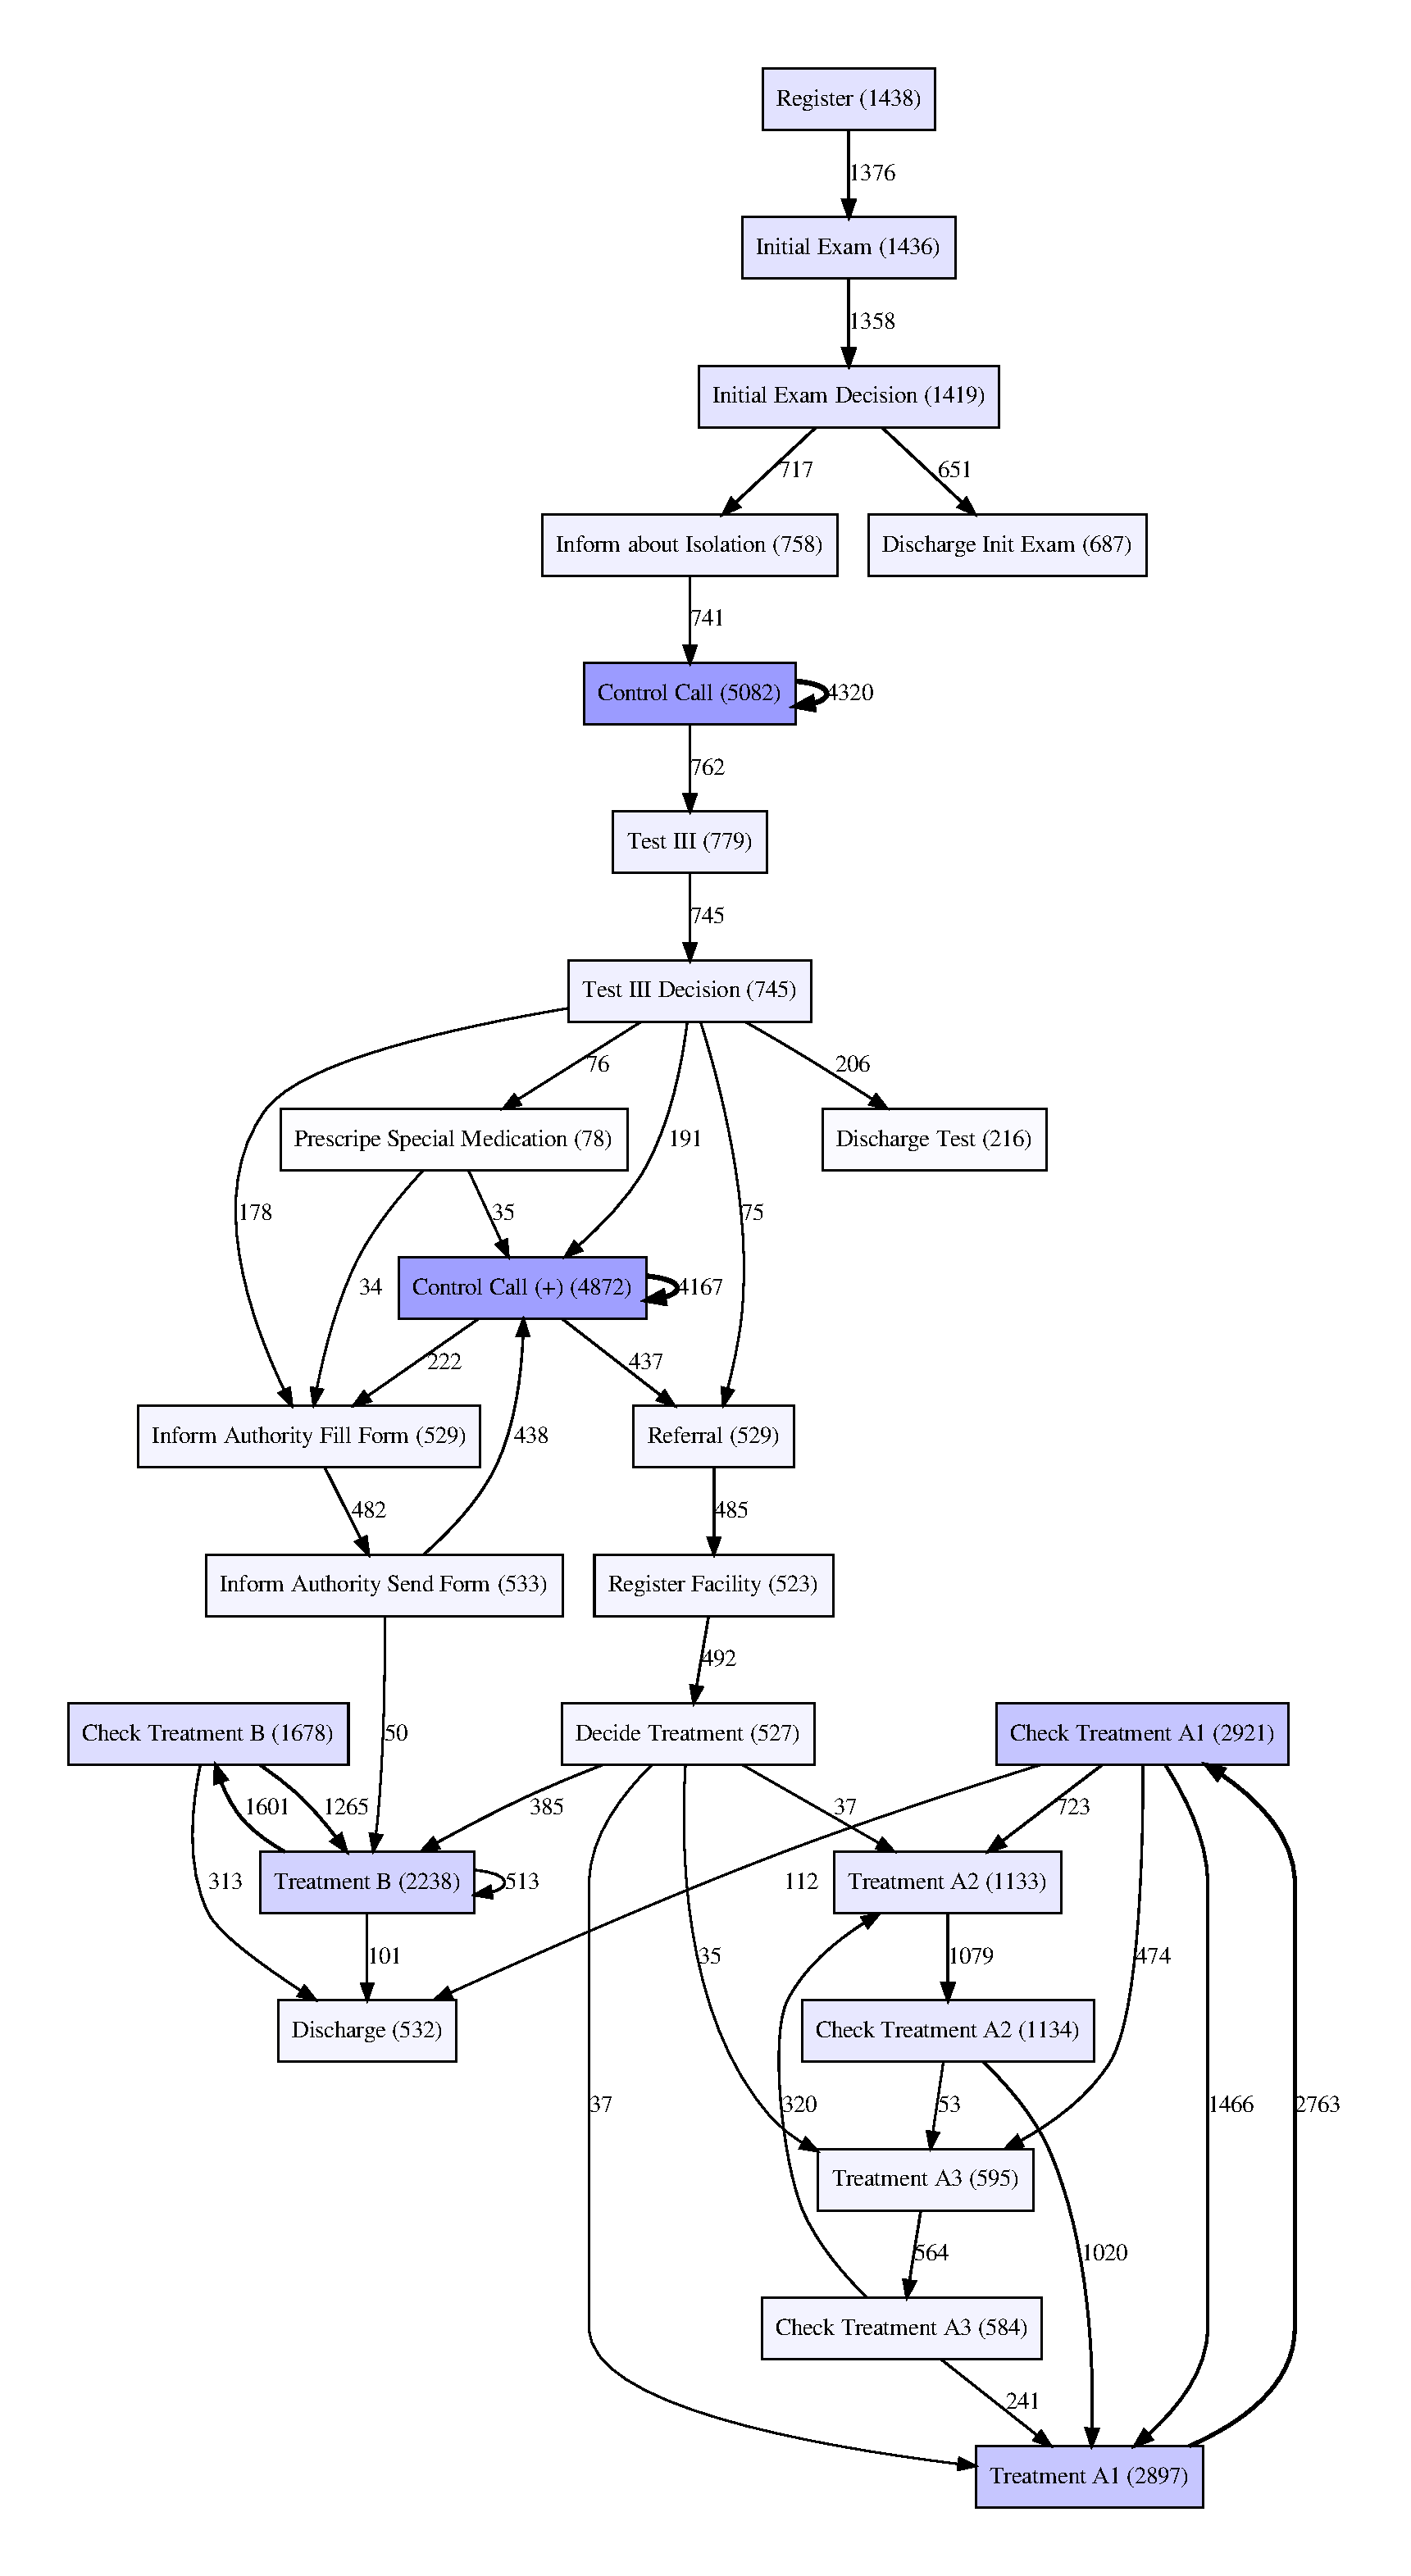
\includegraphics[width=\textwidth]{figures/q1_d_dfg_noise_threshold_tuning.pdf}
        \caption{DFG}
        \label{fig:figures-q1_d_dfg_noise_threshold_tuning-pdf}
    \end{subfigure}
    \hfill
    \begin{subfigure}[b]{0.7\textwidth}
        \centering
	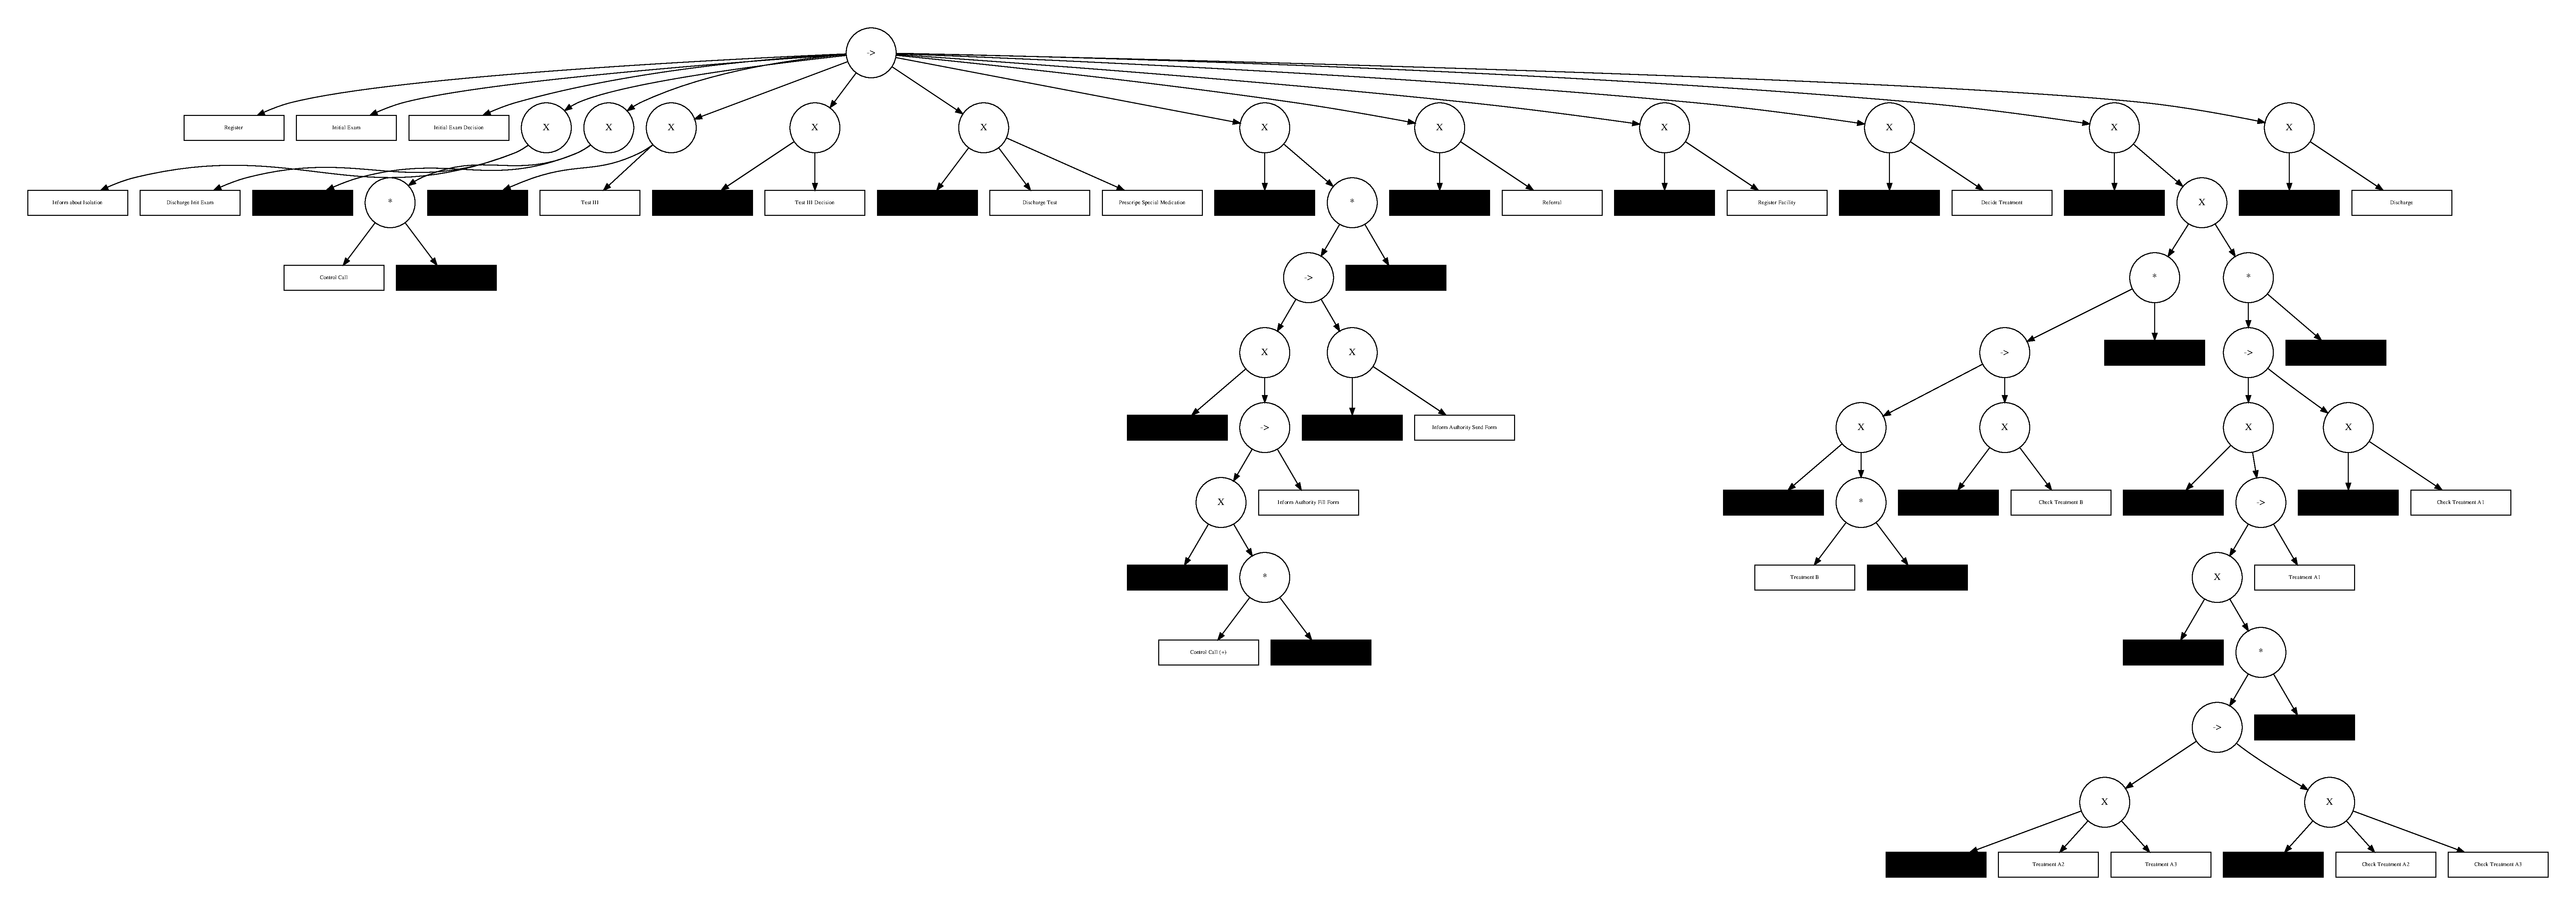
\includegraphics[width=\textwidth]{figures/q1_d_noise_threshold_tuning.pdf}
        \caption{Process Tree}
        \label{fig:q1_d_noise_threshold_tuninig-pdf}
    \end{subfigure}
    \hfill
    \caption{Model resulting from the tuning of the noise threshold}
    \label{fig:noise-threshold-tuning-model}
\end{figure}

\paragraph{e)} 

Analysing the traces in which this activity occur we reinforce what was noted above and estimate that the special medication is prescribe only to patients that go through the A treatments, therefore reasoning its total absence from the model where these traces were filtered out. To try and understand this better, we modeled only these traces that were left out from the aforementioned model. The result can be seen in Figure \ref{fig:special-medication-model}. Besides what was already discussed, one can say that the previous models failed to capture the non-local influence of this activity, which is expected for the Inductive Mining algorithm.

\begin{figure}[h]
    \centering
    \begin{subfigure}[b]{0.2\textwidth}
        \centering
	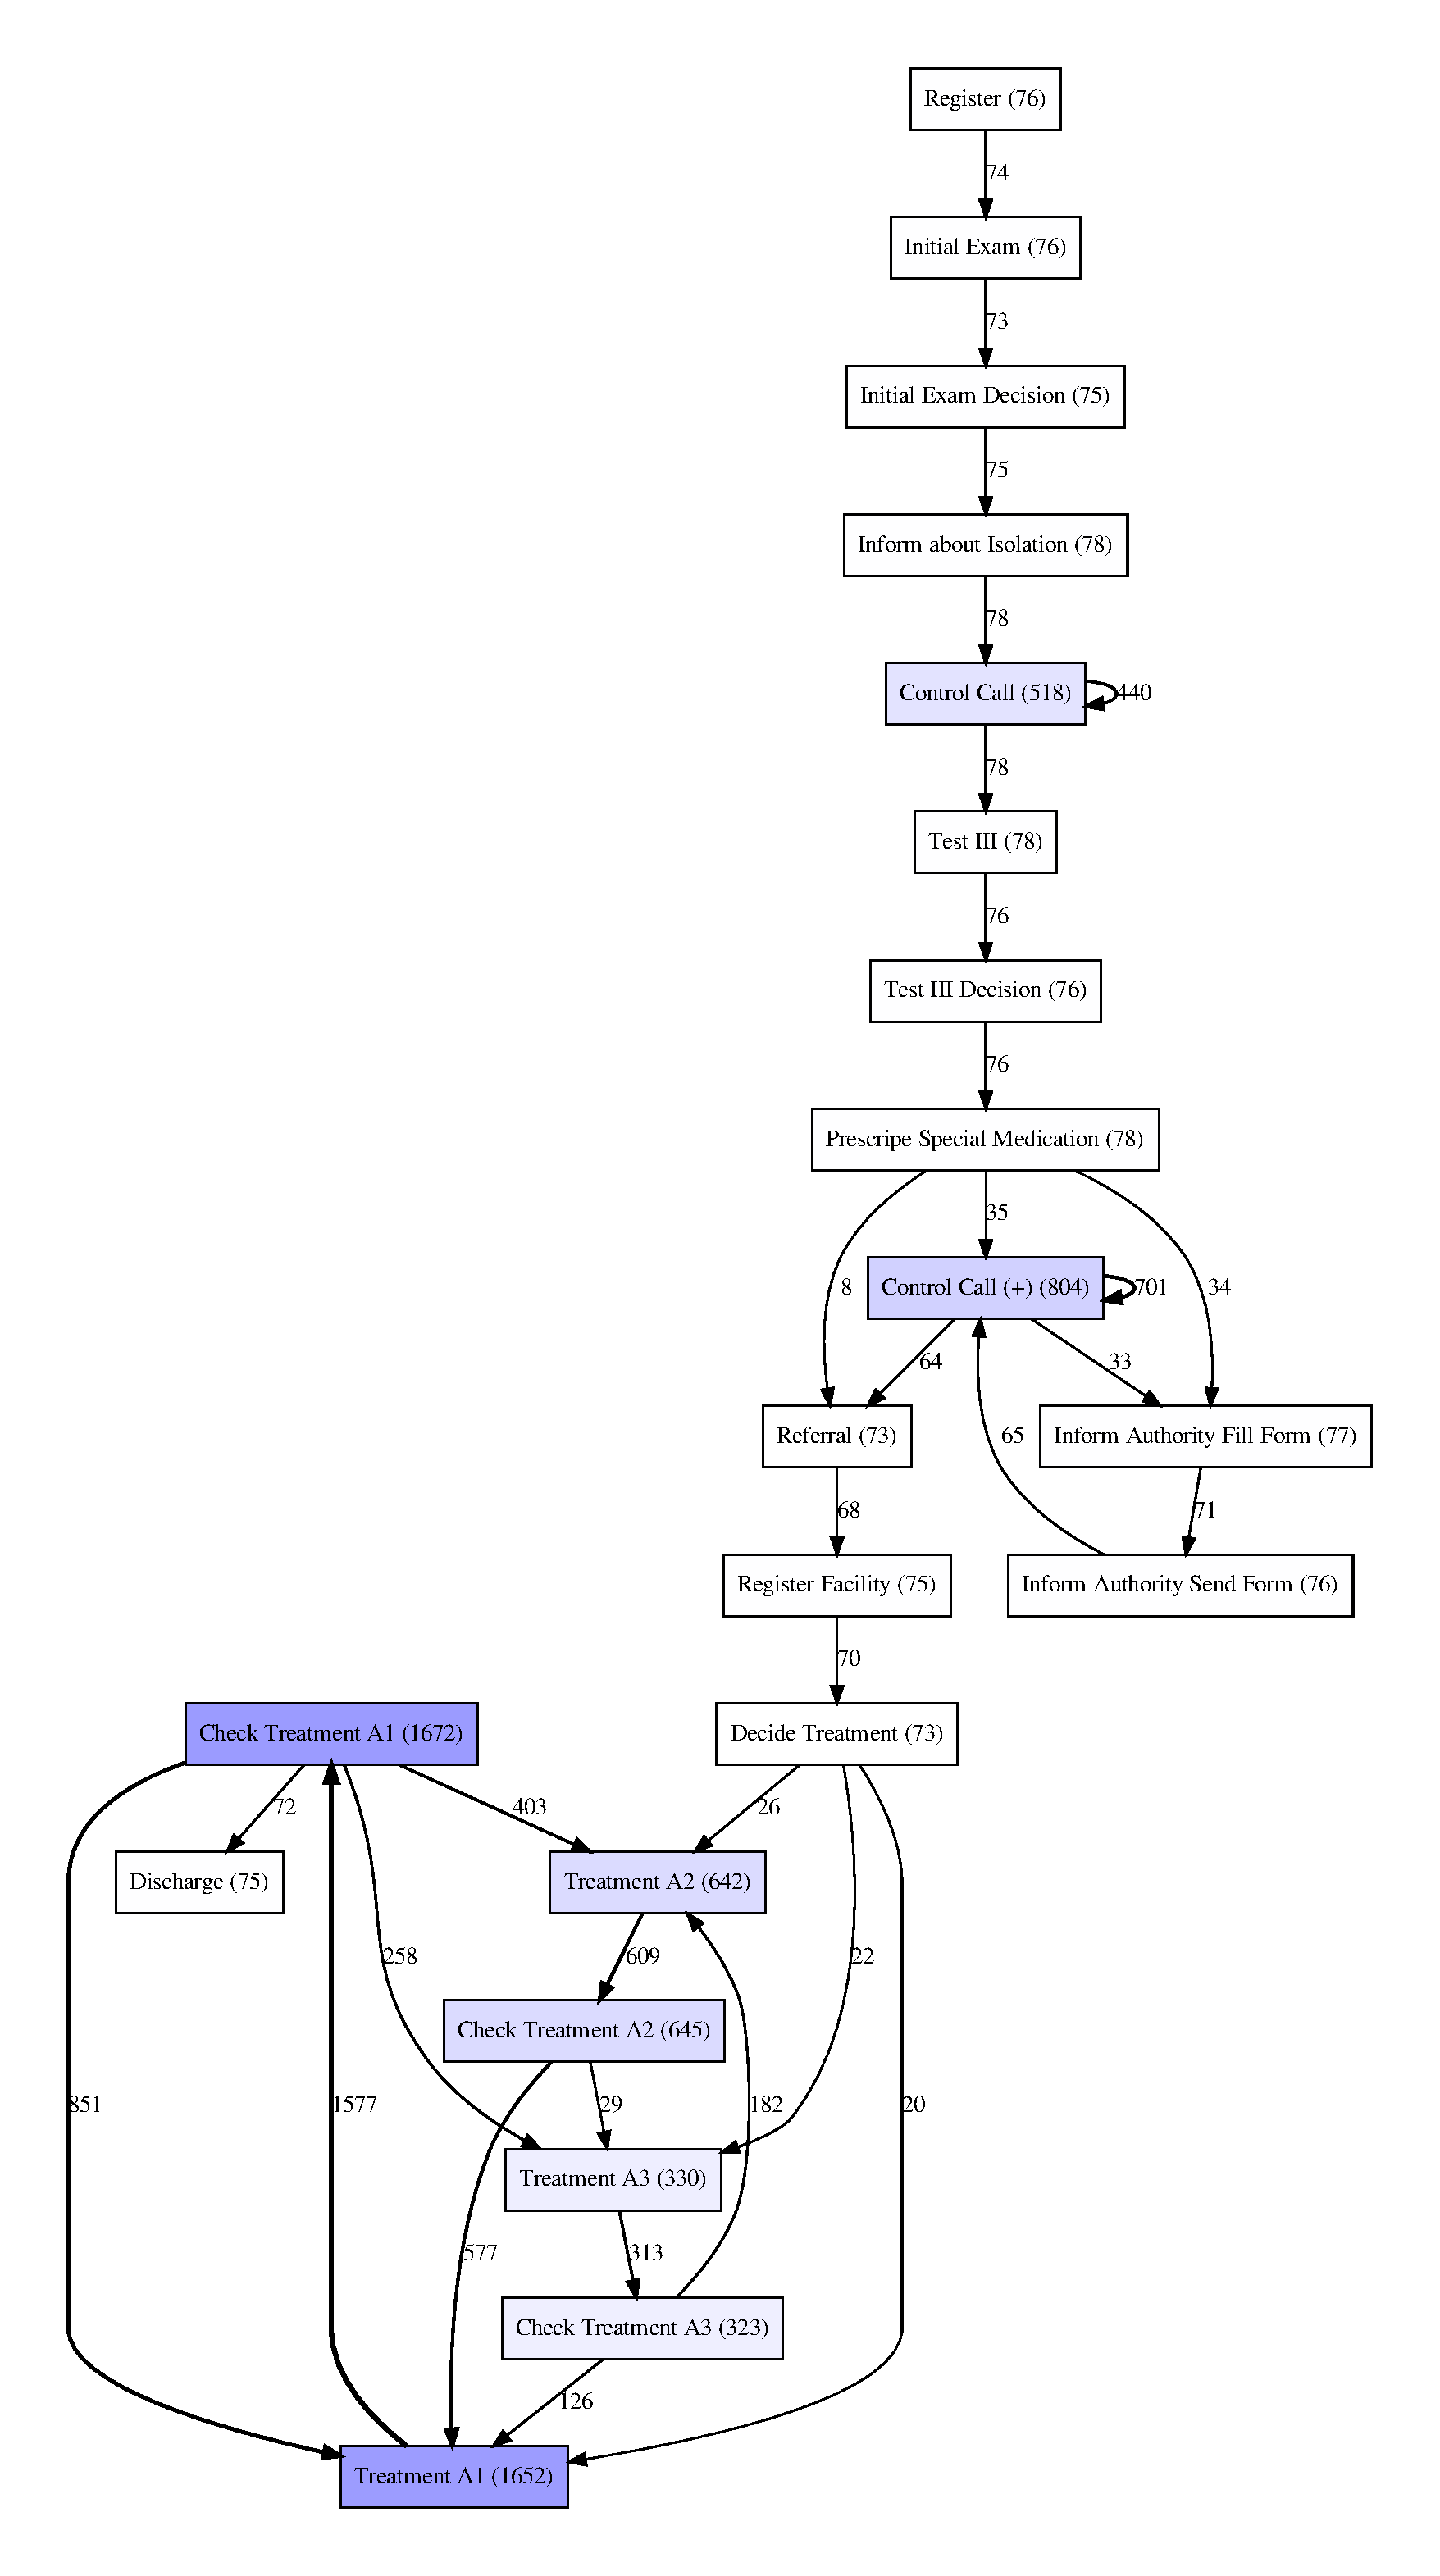
\includegraphics[width=\textwidth]{figures/q1_e_special.pdf}
        \caption{DFG}
        \label{fig:figures-q1_e_special-pdf}
    \end{subfigure}
    \hfill
    \begin{subfigure}[b]{0.7\textwidth}
        \centering
	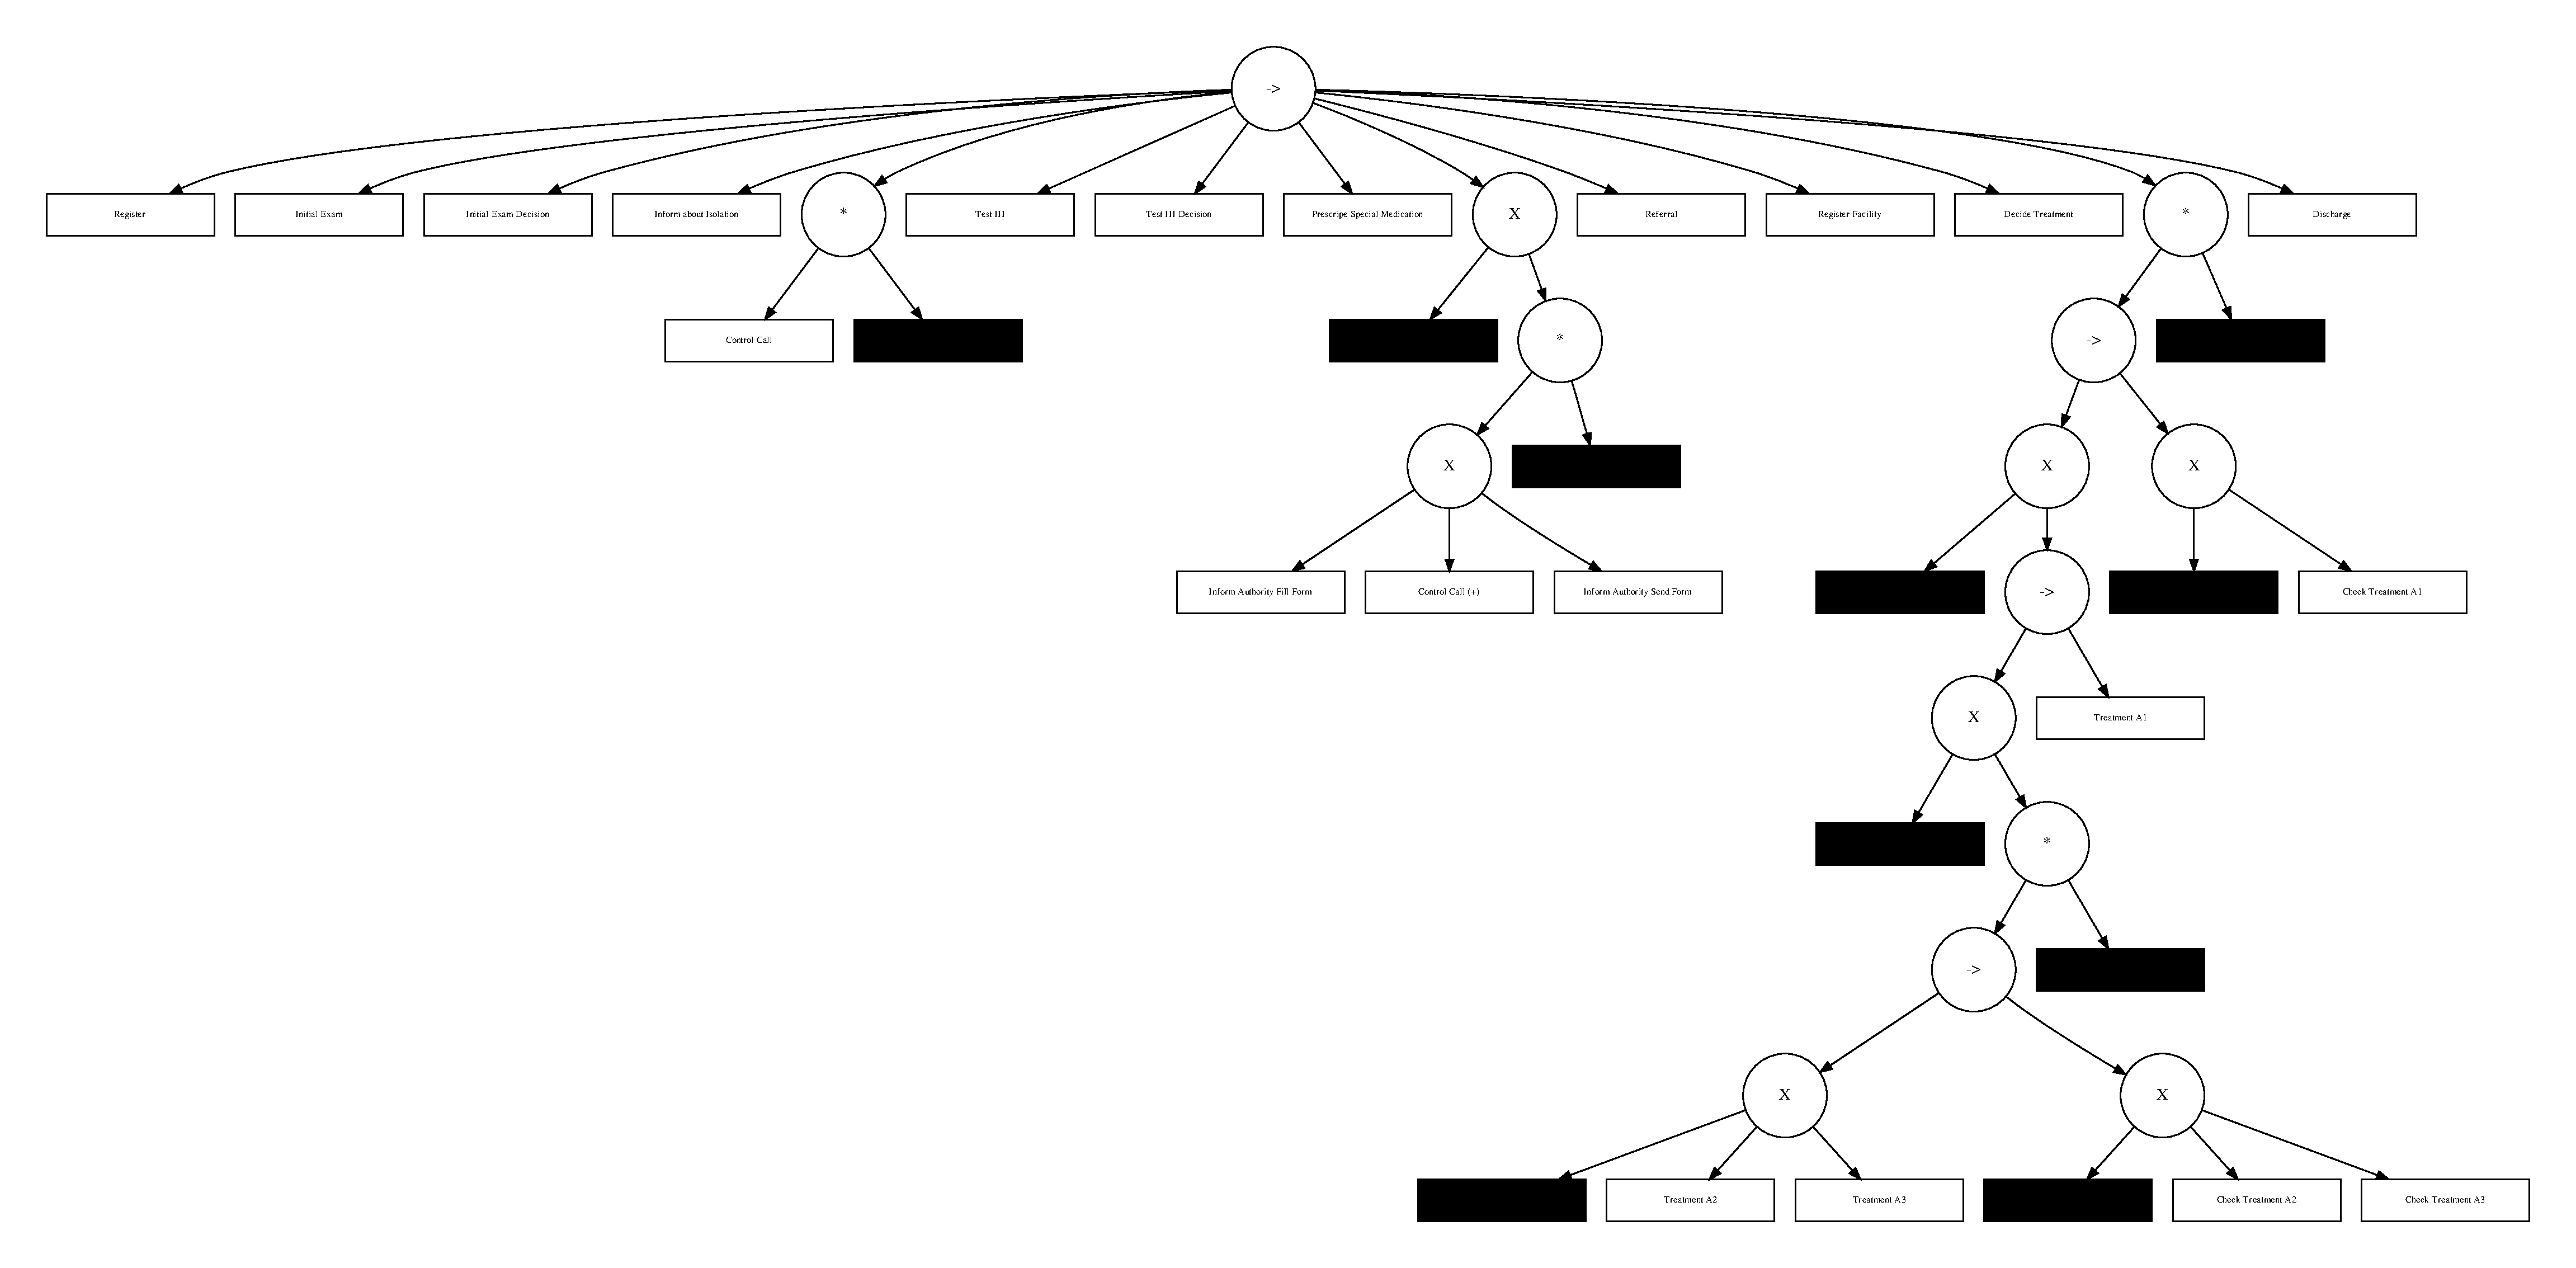
\includegraphics[width=\textwidth]{figures/q1_e_tree_special.pdf}
        \caption{Process Tree}
        \label{fig:q1_e_tree_special-pdf}
    \end{subfigure}
    \hfill
    \caption{Model resulting from event log containing only the traces in which the \emph{Prescripe Special Medication} was present}
    \label{fig:special-medication-model}
\end{figure}

\paragraph{f)} 

The Alpha Miner and the Heuristics Miner algorithms were applied to the event log. The resulting model from the AM can be seen in Figure \ref{fig:figures-q1_f_alpha_miner-pdf}. We can see that the resulting Petri Net fails to model most of the behaviors of the process, having several loose transitions and even failing to be an workflow net.

\begin{figure}[h]
    \centering
    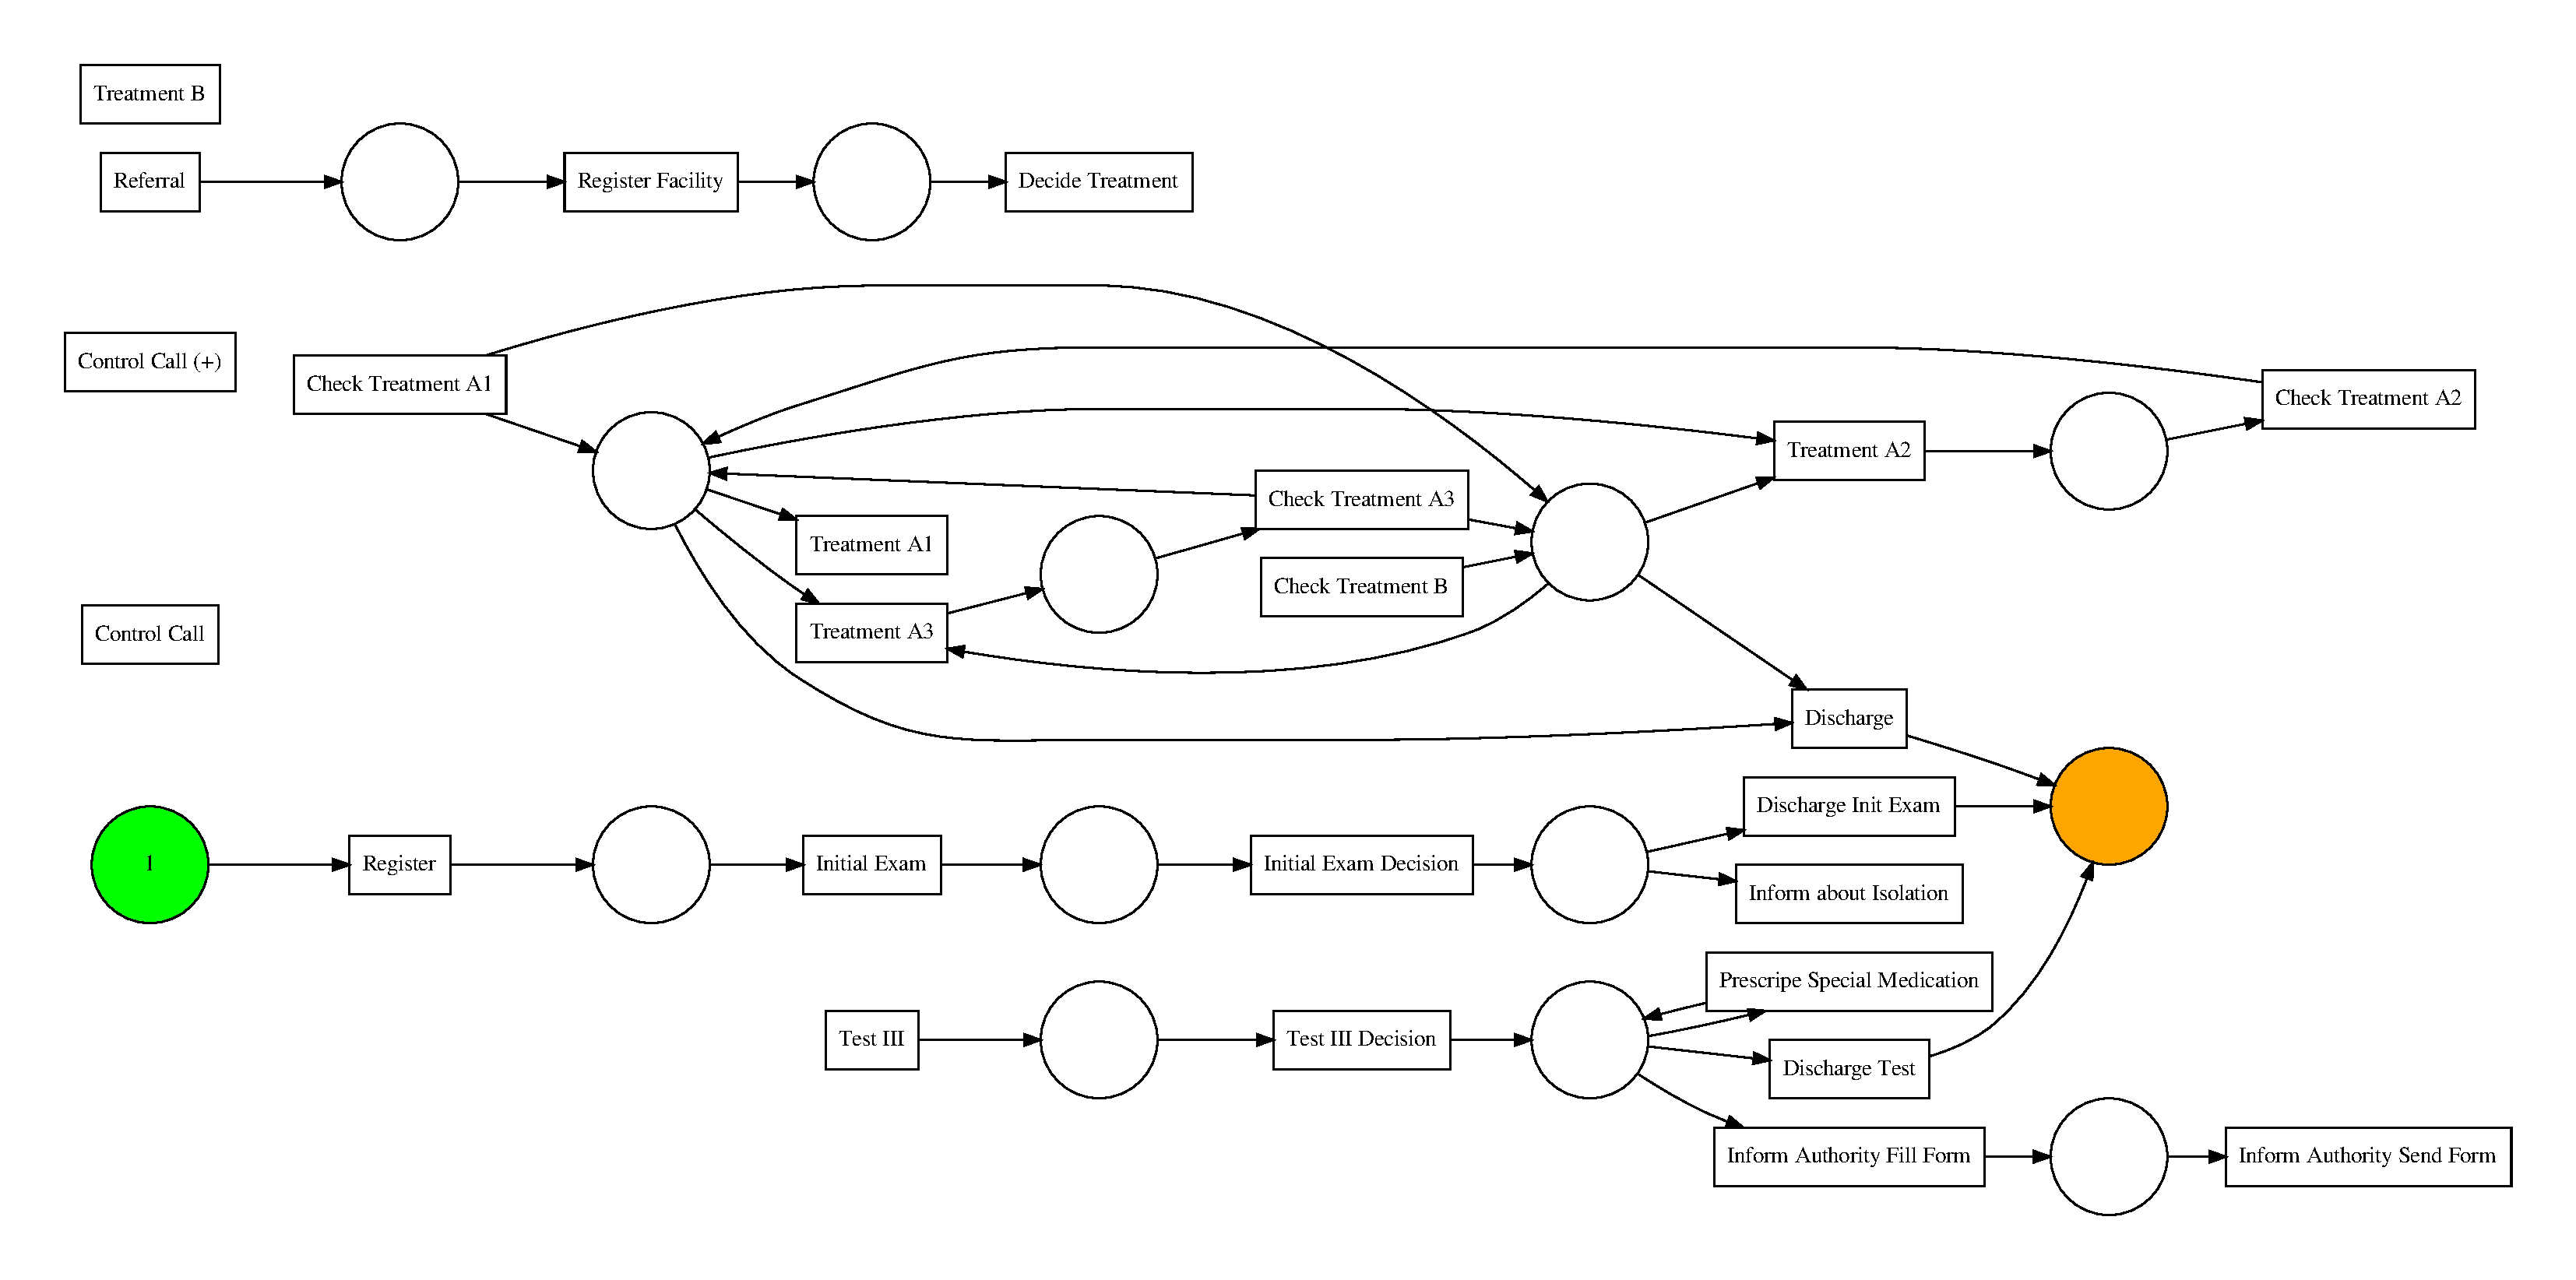
\includegraphics[width=\textwidth]{figures/q1_f_alpha_miner.pdf}
    \caption{Petri Net resulting from the Alpha Miner application to the event log}
    \label{fig:figures-q1_f_alpha_miner-pdf}
\end{figure}

The results of the HM application can be seen in Figure \ref{fig:figures-q1_f_heuristics_miner-pdf}. It presents a satisfactory modeling of the initial activities and even some of the more complex behaviors as the first \emph{Control Call} and the split after the test. But it also fails to model the non-local influence of the \emph{Prescripe Special Medication} activity and the relation between the treatment activities. We also notice that the model is not sound, allowing for the overflow of tokens in some places through silent transitions. Perhaps the biggest problem of this model is related to the activities related to the treatment, where it fails to model the behavior almost completely.

\begin{figure}[h]
    \centering
    
\includegraphics[width=\textwidth]{figures/q1_f_heuristics_miner.pdf}
    \caption{Petri Net resulting from the Heuristics Miner application to the event log}
    \label{fig:figures-q1_f_heuristics_miner-pdf}
\end{figure}

For these, we can conclude that the Inductive Miner presented the best model out of the 3 algorithms tried.

\section{Q2. Social Network Analysis}
\textlangle Optional: Introduction \textrangle
\paragraph{a)} \textlangle Provide the answer here\textrangle
\paragraph{b)} \textlangle Provide the answer here\textrangle
\paragraph{c)} \textlangle Provide the answer here\textrangle
\paragraph{d)} \textlangle Provide the answer here\textrangle

\section{Q3. Performance Analysis}
\textlangle Optional: Introduction \textrangle
\paragraph{a)} \textlangle Provide the answer here\textrangle
\paragraph{b)} \textlangle Provide the answer here\textrangle

\section{Q4. Decision Points}
\textlangle Optional: Introduction \textrangle
\paragraph{a)} \textlangle Provide the answer here\textrangle
\paragraph{b)} \textlangle Provide the answer here\textrangle

\section{Q5. Proccess Improve Suggestions}
\textlangle Optional: Introduction \textrangle \\
\textlangle Provide the answer here\textrangle

\newpage
\section{Appendix}

\end{document}

